\documentclass[preprint,12pt,authoryear]{elsarticle}

\usepackage[T1]{fontenc}
\usepackage[utf8]{inputenc}
\usepackage{lmodern}
\usepackage{booktabs,tabularx,array}
\usepackage{graphicx,float}
\usepackage{xcolor,microtype,url,hyperref}
\usepackage[nameinlink,capitalize,noabbrev]{cleveref}

\graphicspath{{figures/}}
\setlength{\emergencystretch}{3em}
\hypersetup{
  colorlinks=true,
  linkcolor=blue!45!black,
  urlcolor=blue!55!black,
  pdftitle={High-level research overview: shared burst dynamics and neuron identifiability},
  pdfauthor={Raul Valle, Jose Principe, Yinong Chen, Chenyu Liang, Xin Tang}
}

% Shared mathematical notation.
\newcommand{\Y}{\mathbf{Y}}
\newcommand{\X}{\mathbf{X}}
\newcommand{\calX}{\mathcal{X}}
\newcommand{\E}{\mathbb{E}}
\newcommand{\Var}{\operatorname{Var}}
\newcommand{\Cov}{\operatorname{Cov}}
\newcommand{\Corr}{\operatorname{Corr}}
\newcommand{\median}{\operatorname{median}}
\newcommand{\MAD}{\operatorname{MAD}}
\newcommand{\argmax}{\operatorname*{arg\,max}}
\newcommand{\ROI}{\mathrm{ROI}}
\newcommand{\SNR}{\mathrm{SNR}}
\newcommand{\LOBO}{\mathrm{LOBO}}
\newcommand{\LOSO}{\mathrm{LOSO}}
\newcommand{\PU}{\mathrm{PU}}
\newcommand{\dd}{\,\mathrm{d}}

% Draft and provisional-result helpers.
\definecolor{provisionalorange}{RGB}{166,82,0}
\definecolor{draftred}{RGB}{155,25,25}
\newif\ifshowprovisional
\showprovisionaltrue

\newcommand{\Provisional}[1]{%
  \ifshowprovisional
    \textcolor{provisionalorange}{#1}\textsuperscript{\textcolor{provisionalorange}{\ensuremath{\dagger}}}%
  \else
    #1%
  \fi
}
\newcommand{\Missing}[1]{\textcolor{draftred}{[MISSING: #1]}}
\newcommand{\AuthorDecision}[1]{\textcolor{draftred}{[AUTHOR DECISION: #1]}}
\newcommand{\CodexReplace}[1]{\textcolor{draftred}{[CODEX REPLACE: #1]}}
\newcommand{\DraftOnly}[1]{\textcolor{draftred}{#1}}
\newcommand{\DraftBanner}{%
  \begin{center}
  \fcolorbox{draftred}{red!3}{%
  \parbox{0.93\linewidth}{\small\textbf{Complete working manuscript; author review required.}
  Daggered values remain explicitly provisional and are excluded from the main claim path.
  Author, ethics, funding, data-release, and final adjudication fields require review.
  The release build must disable provisional mode and contain no red placeholders.}}
  \end{center}
}

\newcommand{\DraftFigure}[3]{%
\begin{figure}[!htbp]
  \centering
  \fbox{\parbox[c][0.23\textheight][c]{0.90\linewidth}{\centering
  \textbf{Planned figure}\par\medskip #1}}
  \caption{#2}
  \label{#3}
\end{figure}}

\newcommand{\ProvisionalFigure}[4]{%
\begin{figure}[!htbp]
  \centering
  \IfFileExists{figures/#2}{\includegraphics[width=#1]{#2}}{%
    \fbox{\parbox[c][0.20\textheight][c]{0.90\linewidth}{\centering Missing provisional asset: \nolinkurl{#2}}}}
  \caption{#3 \textbf{Provisional:} this artifact predates the identity/geometry repair and is included only to guide the confirmatory rerun.}
  \label{#4}
\end{figure}}

% Generated by scripts/build_results_macros.py; do not edit by hand.
\newcommand{\ResultsGeneratedOn}{2026-08-24}
\newcommand{\ResultsSourceStatus}{pre-repair repository audit}

\newcommand{\CarrierRecallBtwenty}{\Provisional{\ensuremath{0.5409}}}
\newcommand{\CertaintyDominantClassCramersV}{\ensuremath{0.346}}
\newcommand{\CertaintyDominantClassPermutationP}{\ensuremath{0.313}}
\newcommand{\CoherenceRecallBtwenty}{\Provisional{\ensuremath{0.6053}}}
\newcommand{\ICADiffRSquared}{\Provisional{\ensuremath{0.9938}}}
\newcommand{\ICADiffScoreCorrelation}{\Provisional{\ensuremath{0.9988}}}
\newcommand{\ICADiffShiftP}{\Provisional{\ensuremath{0.005}}}
\newcommand{\LagRecallBtwenty}{\Provisional{\ensuremath{0.6220}}}
\newcommand{\LeftRightGlobalCorrelation}{\Provisional{\ensuremath{0.557}}}
\newcommand{\NCurrentBursts}{\Provisional{4}}
\newcommand{\NCurrentCanonicalNeurons}{\Provisional{26}}
\newcommand{\NCurrentOccurrences}{\Provisional{79}}
\newcommand{\NCurrentOriginalSites}{\Provisional{27}}
\newcommand{\NCurrentRecordings}{\Provisional{1}}
\newcommand{\ProvisionalFieldBoundaryX}{\Provisional{\ensuremath{x=286}}}
\newcommand{\QuietVarianceSlope}{\Provisional{\ensuremath{3.63}}}
\newcommand{\QuietVarianceWeightedRtwo}{\Provisional{\ensuremath{0.955\text{--}0.959}}}
\newcommand{\RawAnnulusCIHigh}{\Provisional{\ensuremath{0.0008}}}
\newcommand{\RawAnnulusCILow}{\Provisional{\ensuremath{-0.0277}}}
\newcommand{\RawAnnulusDelta}{\Provisional{\ensuremath{-0.0131}}}
\newcommand{\RawFirstPCVariance}{\Provisional{\ensuremath{87.4\%}}}
\newcommand{\RawHeldoutCorrelation}{\Provisional{\ensuremath{0.8256}}}
\newcommand{\RawWithinSiteMedianCorrelation}{\Provisional{\ensuremath{0.3720}}}
\newcommand{\ResidualHeldoutCorrelation}{\Provisional{\ensuremath{0.5307}}}
\newcommand{\ResidualPeakAmplitudeCIHigh}{\Provisional{\ensuremath{140.75}}}
\newcommand{\ResidualPeakAmplitudeCILow}{\Provisional{\ensuremath{50.64}}}
\newcommand{\ResidualPeakAmplitudeDelta}{\Provisional{\ensuremath{91.33}}}
\newcommand{\ResidualSpatialCIHigh}{\Provisional{\ensuremath{0.0472}}}
\newcommand{\ResidualSpatialCILow}{\Provisional{\ensuremath{-0.2560}}}
\newcommand{\ResidualSpatialDelta}{\Provisional{\ensuremath{-0.0953}}}
\newcommand{\ResidualWithinSiteMedianCorrelation}{\Provisional{\ensuremath{0.3144}}}
\newcommand{\SpatialICAContrastDelta}{\ensuremath{0.170}}
\newcommand{\SpatialICAContrastQ}{\ensuremath{0.0001}}
\newcommand{\SpatialICAMinEventMapCorrelation}{\ensuremath{0.9983}}
\newcommand{\SpatialICAMinMorphologySpearman}{\ensuremath{0.9948}}
\newcommand{\SpatialICAMinPixelCorrelation}{\ensuremath{0.9985}}
\newcommand{\SpatialICAPeakOffsetDelta}{\ensuremath{-3.990}}
\newcommand{\SpatialICAPeakOffsetQ}{\ensuremath{0.0003}}
\newcommand{\SpatialICARadiusDelta}{\ensuremath{-1.335}}
\newcommand{\SpatialICARadiusQ}{\ensuremath{0.0014}}
\newcommand{\SpatialICAReferenceRecall}{\ensuremath{0.6714}}
\newcommand{\SpatialICAVsevenBoundaryEpsilon}{\ensuremath{0.323}}
\newcommand{\SpatialICAVsevenBoundaryQ}{\ensuremath{0.0679}}

% Generated by scripts/import_fig08_full_trace_feature_panel.py; do not edit.
\newcommand{\FullTraceOccurrences}{106}
\newcommand{\FullTraceSites}{50}
\newcommand{\FullTraceCarrierPercentile}{0.994}
\newcommand{\FullTraceCarrierCILow}{0.981}
\newcommand{\FullTraceCarrierCIHigh}{1.000}
\newcommand{\FullTraceCoherencePercentile}{0.994}
\newcommand{\FullTraceLagPercentile}{0.996}
\newcommand{\FullTraceLagDelta}{+0.002}
\newcommand{\FullTraceLagDeltaLow}{0.000}
\newcommand{\FullTraceLagDeltaHigh}{0.006}
\newcommand{\FullTraceRawPercentile}{0.991}
\newcommand{\FullTraceConsensusPercentile}{0.986}
\newcommand{\FullTraceConsensusRepeatability}{0.633}
\newcommand{\FullTracePersistencePercentile}{0.972}
\newcommand{\FullTracePersistenceRepeatability}{0.649}
\newcommand{\FullTraceVSTPercentile}{0.883}
\newcommand{\FullTraceCarrierCeilingCount}{104}
\newcommand{\FullTraceCoherenceCeilingCount}{104}
\newcommand{\FullTraceLagCeilingCount}{105}

% Generated by scripts/import_fig09_automated_feature_validation.py; do not edit.
\newcommand{\AutoRawAUC}{0.931}
\newcommand{\AutoRawAUCLow}{0.906}
\newcommand{\AutoRawAUCHigh}{0.952}
\newcommand{\AutoCarrierAUC}{0.920}
\newcommand{\AutoCoherenceAUC}{0.915}
\newcommand{\AutoLagAUC}{0.905}
\newcommand{\AutoMatchedAUC}{0.884}
\newcommand{\AutoPersistenceSpatialDelta}{0.217}
\newcommand{\AutoRecoveryCount}{94}
\newcommand{\AutoRecoveryMisses}{12}
\newcommand{\AutoCarrierLogLoss}{0.712}
\newcommand{\AutoExtendedLogLoss}{0.577}
\newcommand{\AutoRecoveryDelta}{0.136}
\newcommand{\AutoRecoveryDeltaLow}{-0.025}
\newcommand{\AutoRecoveryDeltaHigh}{0.280}
\newcommand{\AutoCarrierReliability}{0.580}
\newcommand{\AutoAnnulusReliability}{0.866}
\newcommand{\AutoNullP}{0.0020}

% Generated by scripts/import_fig11_feature_deep_dives.py; do not edit.
\newcommand{\DeepRecoveredAll}{83}
\newcommand{\DeepRecoveredPartial}{11}
\newcommand{\DeepAllMisses}{12}
\newcommand{\DeepCoherenceNativeTwenty}{0.064}
\newcommand{\DeepCoherenceRankingTwenty}{0.011}
\newcommand{\DeepLagNativeTwenty}{0.081}
\newcommand{\DeepLagRankingTwenty}{0.011}
\newcommand{\DeepKineticKernel}{rise1\_decay20}
\newcommand{\DeepKineticAUC}{0.893}
\newcommand{\DeepKineticLOBOAUC}{0.915}
\newcommand{\DeepCarrierLoss}{0.710}
\newcommand{\DeepCompactLoss}{0.691}


\journal{Research overview accompanying the technical manuscript}

\begin{document}
\begin{frontmatter}

\title{What the current zebrafish fluorescence recording tells us about shared bursts and neuron identifiability}

\author[uf]{Raul Valle}
\author[affpending]{Jose Principe}
\author[affpending]{Yinong Chen}
\author[affpending]{Chenyu Liang}
\author[affpending]{Xin Tang}

\affiliation[uf]{organization={Department of Electrical and Computer Engineering, University of Florida},
  city={Gainesville}, state={Florida}, country={United States}}
\affiliation[affpending]{organization={Affiliations pending author confirmation}}

\begin{abstract}
This document is a reader-friendly companion to the evidence-complete technical
manuscript. The central result is that the recording contains a strong,
repeatable burst waveform, but that waveform is shared by labeled neurons and
nearby tissue. The processing pipeline separates temporal components and
standardizes each location against its local space--time variability. These
transformations produce stable, useful measurement representations, but they do
not by themselves prove that each output is an independently identified neuron.
Across 106 confirmed neuron--burst observations at 50 fixed spatial sites,
complete-trace event localization is already near ceiling for Raw amplitude,
the frozen carrier, local coherence, and lagged recurrence. A harder frame-level
test ranks Raw highest (AUC \AutoRawAUC{}), and all six compact features score
higher at true centers than at matched displaced tissue. A richer recovery
model improves cross-fitted point estimates but does not pass the site-bootstrap
uncertainty gate. Neighborhood coherence adds its clearest value during
full-field candidate ranking. Two
recurrent trace phenotypes summarize major differences in persistence, local
contrast, and spatial coupling. The frozen six-component CS--Parzen temporal ICA
is numerically invertible, and the subsequent local-standardization denominator
has now been reproduced directly at every site. Its global floor was inactive at
all audited centers, showing that center-trace scaling was driven by measured
local variability rather than floor clipping. The study therefore supports an
identifiability-first interpretation: the pipeline is role-specific feature
engineering and a useful detector representation, while biological source identity and
full-field precision remain open validation questions.
\end{abstract}

\begin{keyword}
zebrafish \sep fluorescence imaging \sep feature engineering \sep independent component analysis \sep local standardization \sep identifiability
\end{keyword}

\end{frontmatter}

\DraftBanner
\section{The research question}

The practical question is simple: when the movie becomes brighter during a
burst, how much of that signal belongs to a particular neuron, and how much is a
shared property of the recording or its local neighborhood? This distinction
matters because a visually convincing trace can still reflect neuropil,
illumination, motion, broad recruitment, or several neurons at once.

The current dataset contains four burst intervals and 106 confirmed
neuron--burst observations at 50 coordinate-defined sites. The labels are
sparse positives: a confirmed site is a positive example, but an unlabeled
candidate is not automatically a negative. Consequently, the analysis can
measure recovery of known positives, signal fidelity, spatial localization,
and reproducibility. It cannot estimate full-field precision until a bounded
region receives exhaustive review.

\section{What the pipeline does}

The three displayed stages answer different measurement questions:

\begin{enumerate}
  \item \textbf{Raw fluorescence} preserves the acquired intensity and the
  shared burst waveform.
  \item \textbf{Temporal ICA} applies a frozen six-component delay transform at
  lags 0, 1, 2, 4, 8, and 16 frames. Components 2--5 are combined as the
  residual-energy representation used here.
  \item \textbf{Local standardization} compares that representation with a
  causal local space--time reference. Large output means large signal relative
  to the variability recently observed around that location; it does not mean
  ``probability of being a neuron.''
\end{enumerate}

The representative panels keep the movie and center trace synchronized so that
spatial appearance and temporal behavior can be judged together
(\Cref{fig:overview-cases}). The hero, hard antihero, and seeded random case are
illustrative rather than a performance estimate.

\begin{figure}[p]
  \centering
  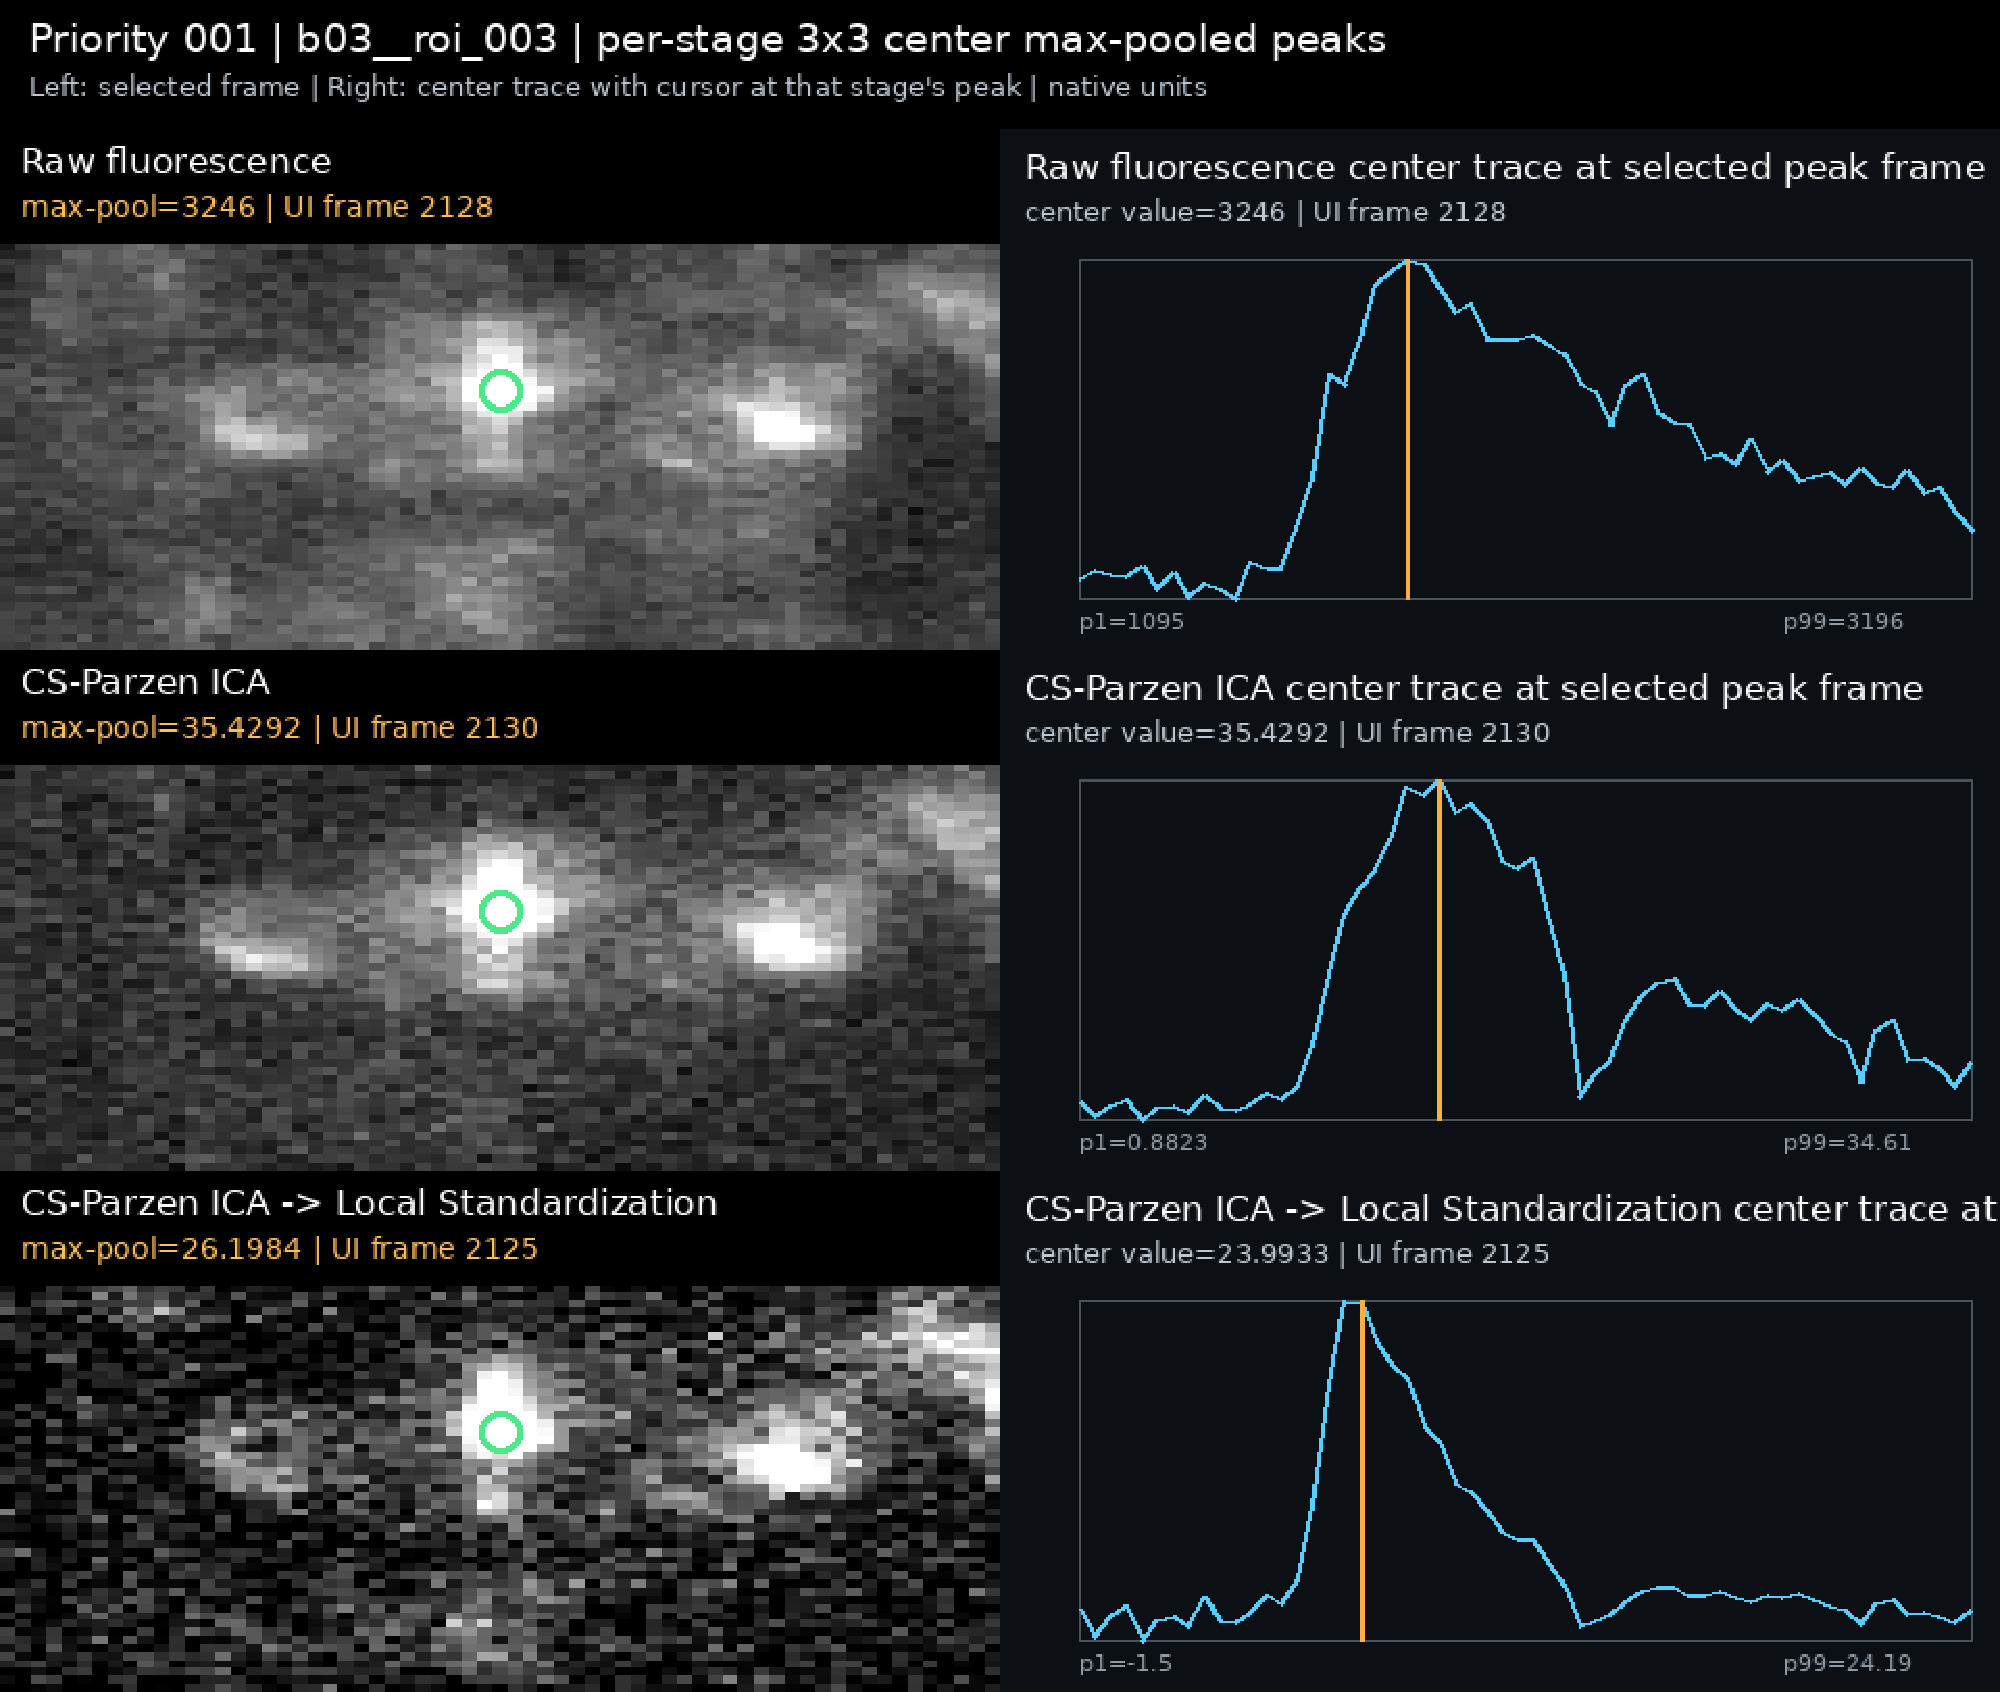
\includegraphics[width=0.96\linewidth,page=1]{figures/final/fig03_trace_atlas_examples.pdf}
  \caption{Representative six-panel review page. Raw, temporal-ICA, and
  local-standardization images are paired with their synchronized ROI-center
  traces. The full technical manuscript includes the hero, antihero, and random
  pages and their frozen selection rules.}
  \label{fig:overview-cases}
\end{figure}

\section{What is established in the current recording}

\begin{table}[H]
\centering
\small
\begin{tabularx}{\linewidth}{>{\bfseries}p{0.20\linewidth} X p{0.22\linewidth}}
\toprule
Claim & Current interpretation & Status and scope \\
\midrule
Shared Burst Waveform & Raw traces contain a strong event-aligned population waveform that is also expressed in nearby tissue. & established\_current\_recording: 106 confirmed occurrences at 50 sites in one recording. \\
Trace Phenotypes & Two descriptive trace phenotypes summarize recurrent within-recording variation. & exploratory: T1 has 38 sites and T2 has 12 sites; these are not biological neuron types. \\
Full Trace Feature Roles & Event amplitude is strongest for known-center temporal retrieval, while spatial context contributes localized structure and full-field proposal or ranking value. & exploratory\_supported\_current\_recording: 106 confirmed occurrences at 50 immutable sites in one previously analyzed recording; displaced tissue and guarded quiet frames have unknown biology. \\
Automated Feature Complementarity & A role-specific feature set improves cross-fitted detector-recovery point estimates over a carrier-only model, but the site-bootstrap uncertainty gate is not passed. & exploratory\_unresolved: 94 recovered and 12 missed original geometries at detector budget 58; site-bootstrap log-loss improvement interval crosses zero. \\
Feature Role Decomposition & Early-budget coherence and lag gains are larger in native proposal streams than on a common proposal universe, while a fixed kinetic filter and lag add distinct exploratory recovery value. & exploratory\_supported\_current\_recording: 106 occurrences at 50 immutable sites; 12 all-lane B58 misses; 20 repeated site-grouped splits and four leave-one-burst-out kinetic folds. \\
Identity Aware Miss Interpretation & Most apparent local recentering improvements among the all-lane misses cross an existing identity boundary and therefore cannot be treated as safe coordinate corrections. & established\_reviewed\_current\_recording: Canonical-v8 interpretation audit of the 12 canonical-v7 all-lane B58 misses; 2 same-identity collisions, 6 other-identity collisions, and 4 identity-clear hypotheses under a fixed six-pixel guard. \\
Expanded Automated Feature Validation & Identity-grouped recovery prediction, stability selection, conditional importance, selective risk, and recovered-only anomaly detection support a compact observability-context stack beyond carrier amplitude alone. & exploratory\_supported\_current\_recording: 106 occurrences at 50 sites in one recording; 12 misses; 100 site-bootstrap sparse fits; synthetic tests are one-dimensional and cross-burst transfer has only one identity-clear pair. \\
Realistic Movie Spatial Context & Spatial context improves source-pixel discrimination over pixel variance in a paired truth-known movie stress test spanning proximity, amplitude imbalance, temporal correlation, and non-circular footprints. & established\_computational\_simulation: 432 paired simulator cells across 12 seeds; mean AUC gain 0.104 and 94.9 percent win fraction; not biological external validation. \\
Realistic Movie Detector Roles & In exact-truth movie detection, the combined carrier-context-kinetic stack improves compact-budget identity recovery and held-seed calibration, while spatial context most strongly improves localization and duplicate suppression. & established\_computational\_simulation: 432 movies, four frozen score stacks, proposal budgets 2, 4, and 8, three-pixel one-to-one identity matching; simulation is not biological transfer. \\
Generator Family Robustness & Spatial context is the most robust frozen proposal score under held-out neuropil, bleaching, nonrigid-motion, empirical-noise, and compound-shift generator families, whereas naive equal-weight fusion retains better calibration but loses operating-point robustness. & established\_computational\_simulation: 108 exact-truth movies across six generator families, six seeds per family, and source counts 2, 4, and 8; empirical noise scale estimated label-free from one untouched 060126 recording. \\
Prospective Gated Fusion & A development-family-trained gated fusion does not improve aggregate F1 over frozen spatial context when thresholds are calibrated without labels on source-free development movies and evaluated on untouched generator families. & established\_computational\_negative\_result: 54 untouched-family movies with 2, 4, or 8 sources; three development families for gate fitting and null calibration; target false-alarm rates 1, 2, and 4 per movie. \\
Automated Challenge Boundaries & A twelve-family exact-truth challenge suite identifies spatial-context robustness alongside concrete limits in weak-neighbor identifiability, deployable stopping, parameter stability, and kinetic direction selectivity. & established\_computational\_mixed\_result: Six seeds per condition across null normalization, suppression, source-count stopping, weak-neighbor, colored noise, motion, morphology, severity, OOD, cross-simulator, stability, and negative-control tests. \\
Targeted V8 Rejections & Parameter-consensus stopping, unconstrained rank-two NMF deblending, and a simple forward-minus-reverse kinetic contrast do not improve their frozen comparators under prospective exact-truth tests. & established\_computational\_negative\_result: Six-seed targeted development package with disjoint artifact definitions, one-to-one weak-identity matching, and explicit forward and reversed kinetic gates. \\
Constrained Generative Rejection & A frozen constrained joint spatial-temporal factorization does not improve close-source identity recovery over spatial context, and component-specific forward-versus-reversed likelihoods remain non-directional after circularity-safe auditing. & established\_computational\_negative\_result: New ellipse development grid followed by one-shot locked v8 crescent evaluation; six seeds; corrected kinetic audit uses unconstrained component coefficients. \\
Temporal Transform Invertibility & The frozen six-component temporal transform is numerically invertible at the audited sites. & established\_computational: Maximum sitewise embedding inversion RMS is 5.69e-12; this is not denoising validation. \\
Ls Denominator Behavior & Local-standardization scaling at audited centers is governed by measured local variability rather than the global floor. & established\_audited\_centers: 50 centers over 560 frames; no full-field floor-inactivity claim. \\
Biological Source Identity & Pipeline outputs identify one-to-one biological neuronal sources. & unresolved: Stable measurement representations do not establish biological source identity. \\
Full Field Precision & Full-field detection precision is known. & unresolved: Sparse positives do not make unmatched candidates verified negatives. \\
New Candidate Single Reviewer Labels & Review of previously unmatched candidates expands the provisional appearance envelope to include small, discreet, low-SNR, and crescent-shaped neuron calls, while artifact-adjacent and neighbor-confounded sites remain unresolved. & provisional\_single\_reviewer: 18 selected unmatched sites in one recording; 9 definite, 4 probable, 4 uncertain, and 1 artifact-or-noise call; no existing decisions changed. \\
External Bounded Review Readiness & A staged portable Raw-first then assisted review package is ready for two independent reviewers, with public/private separation, locked exports, blinding checks, agreement analysis, and mandatory adjudication. & implementation\_complete\_human\_evidence\_pending: One frozen enriched 192 by 192 region and 18 assisted candidates in the current recording; no independent annotations or detector metric yet. \\
\bottomrule
\end{tabularx}
\caption{Generated current-state claim ledger. Status is scoped to the stated evidence boundary.}
\label{tab:overview-status}
\end{table}


\subsection{Population traces and descriptive phenotypes}

The compact population summary shows both the dominant shared waveform and the
heterogeneity hidden by a global average (\Cref{fig:overview-population}). T1
and T2 are measurement phenotypes, not claimed neuron types. Their recurrence
suggests useful structure for diagnostics and feature engineering, while their
biological meaning requires independent recordings and stronger identity
evidence.

\begin{figure}[p]
  \centering
  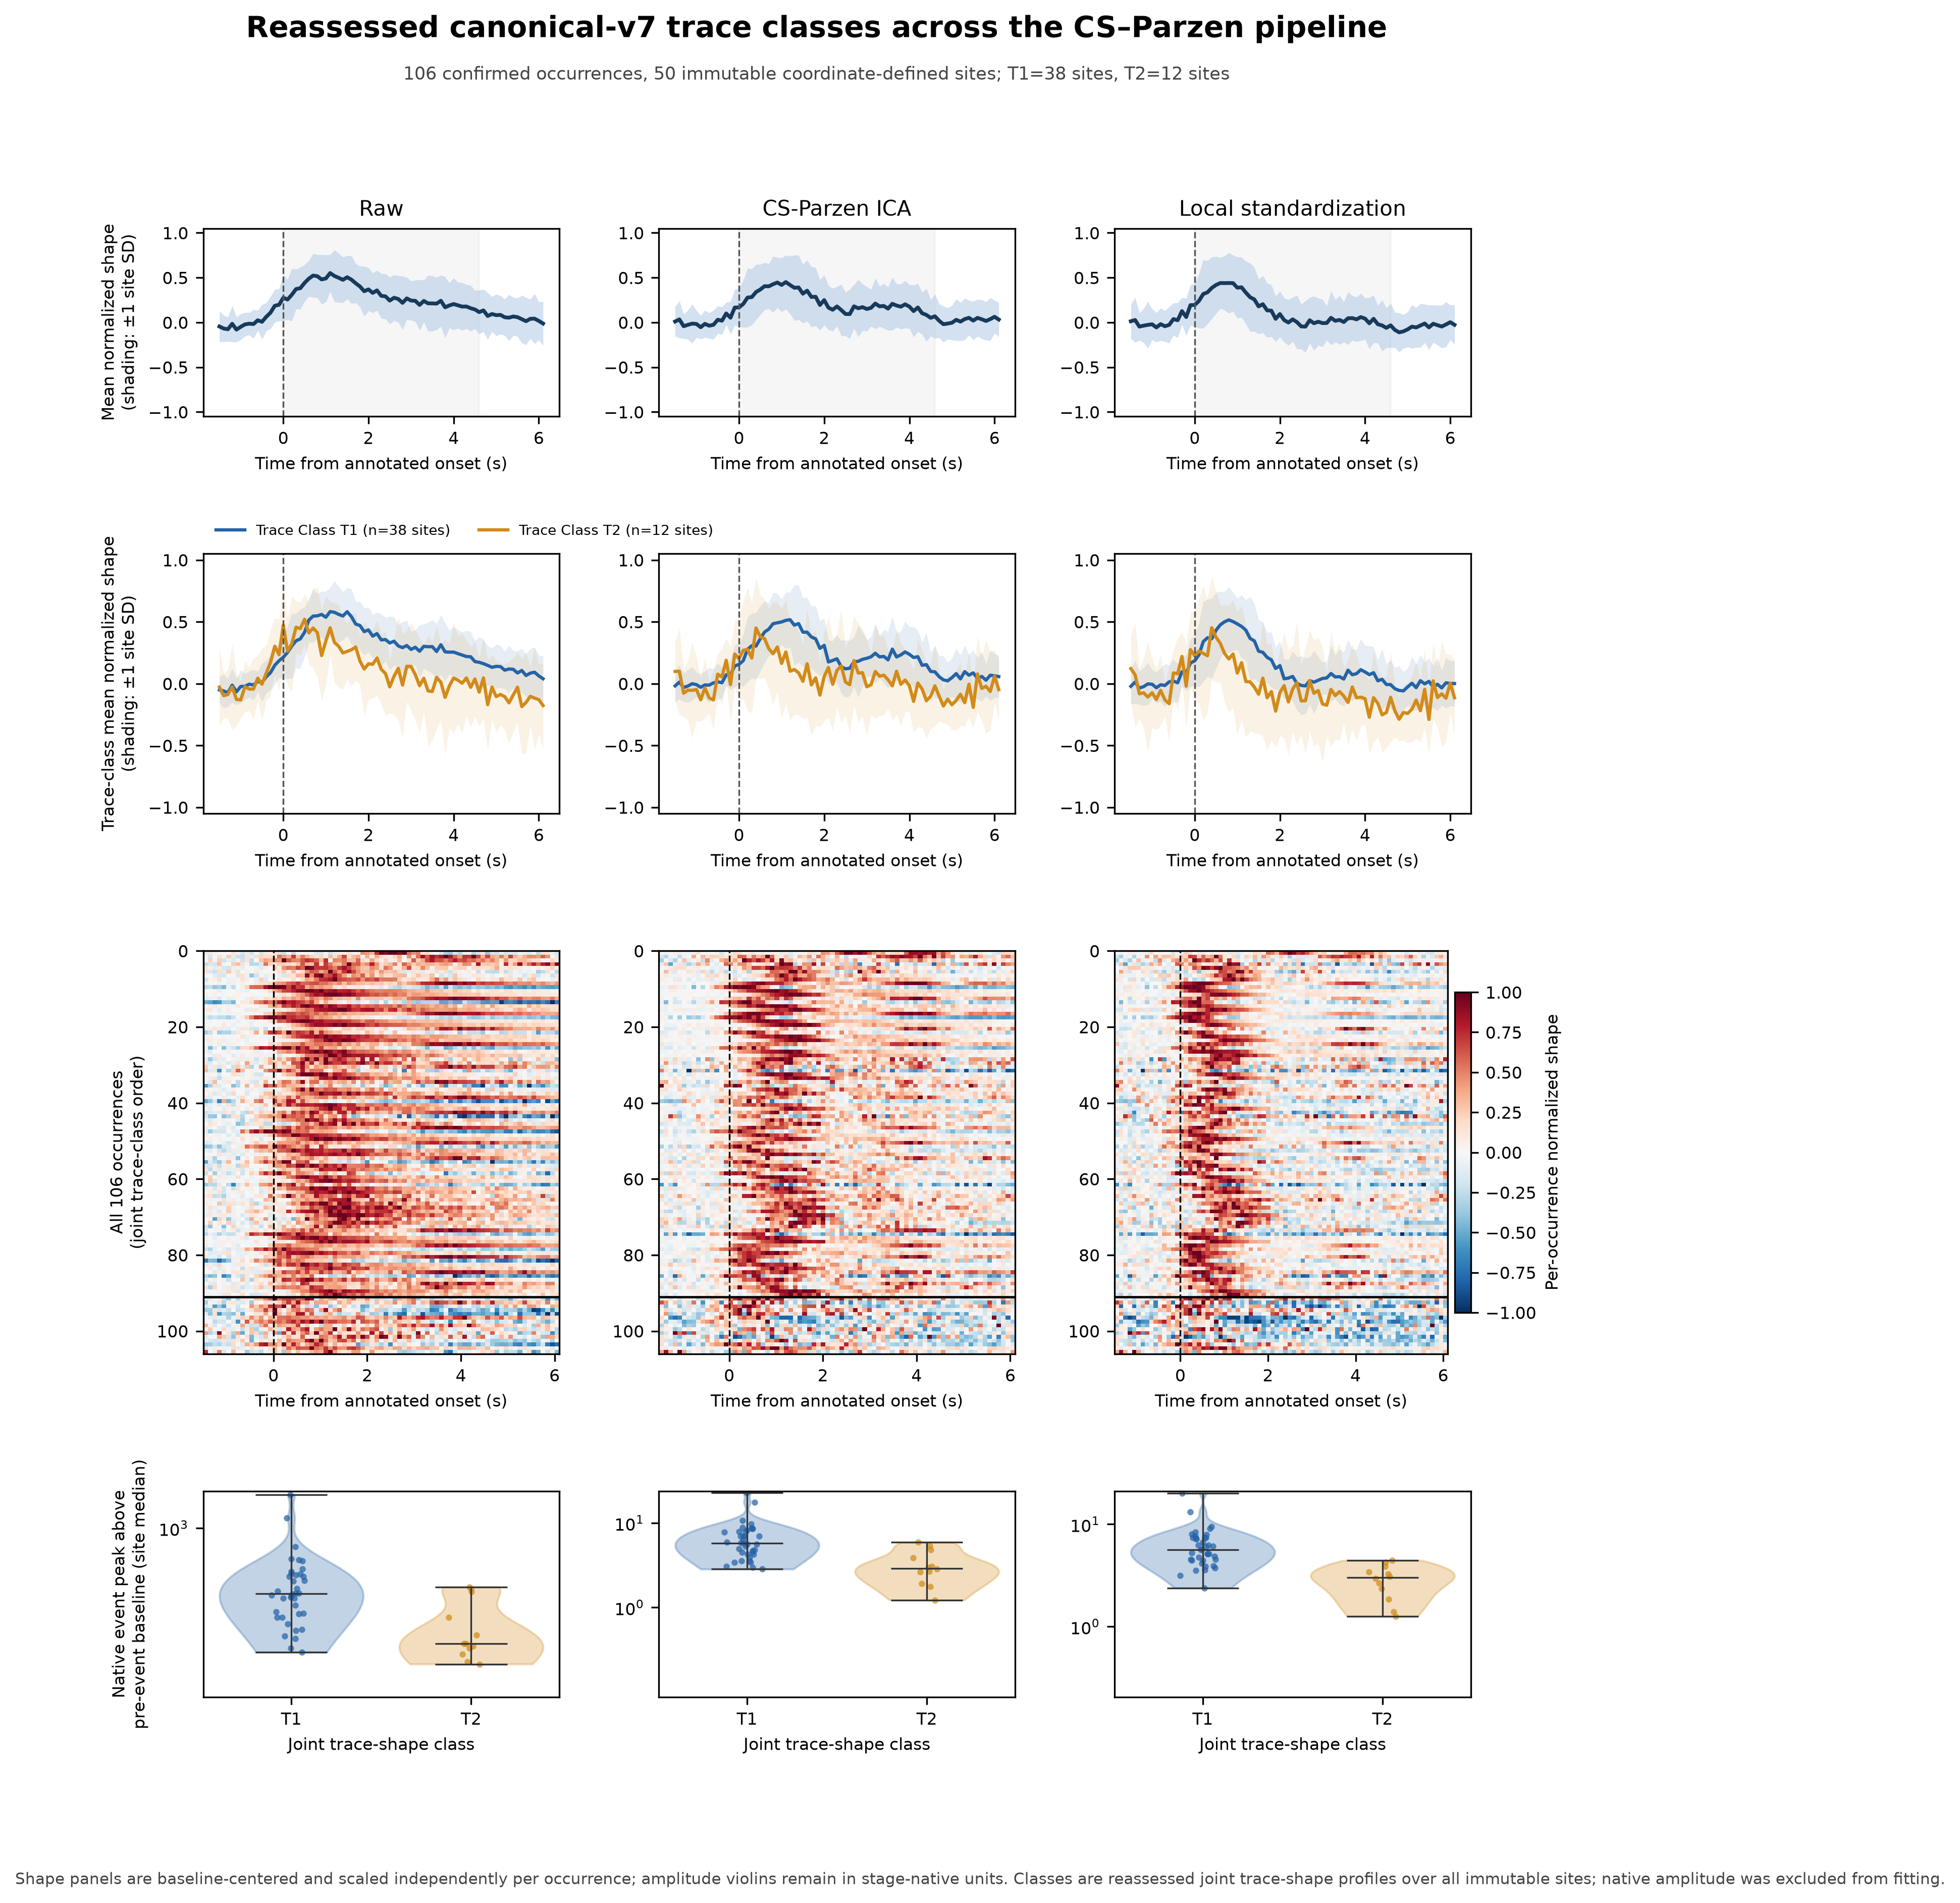
\includegraphics[width=0.98\linewidth]{figures/final/fig04_population_trace_summary.png}
  \caption{Population trace summary across Raw, temporal ICA, and local
  standardization. Global summaries emphasize shared behavior; fixed T1/T2
  summaries expose recurrent differences without asserting biological classes.}
  \label{fig:overview-population}
\end{figure}

\subsection{The diagnostic audit}

The audit combines temporal signal quality, neighborhood coupling, spatial
compactness, stage-transition fidelity, and artifact availability
(\Cref{fig:overview-audit}). It shows that Raw-to-ICA is the larger
transformation, whereas ICA-to-local-standardization preserves trace shape more
closely. Burst 2 remains a weaker and timing-sensitive condition. Candidate
metadata cover only part of the confirmed occurrence set, and independent
recording validation remains unavailable.

\begin{figure}[p]
  \centering
  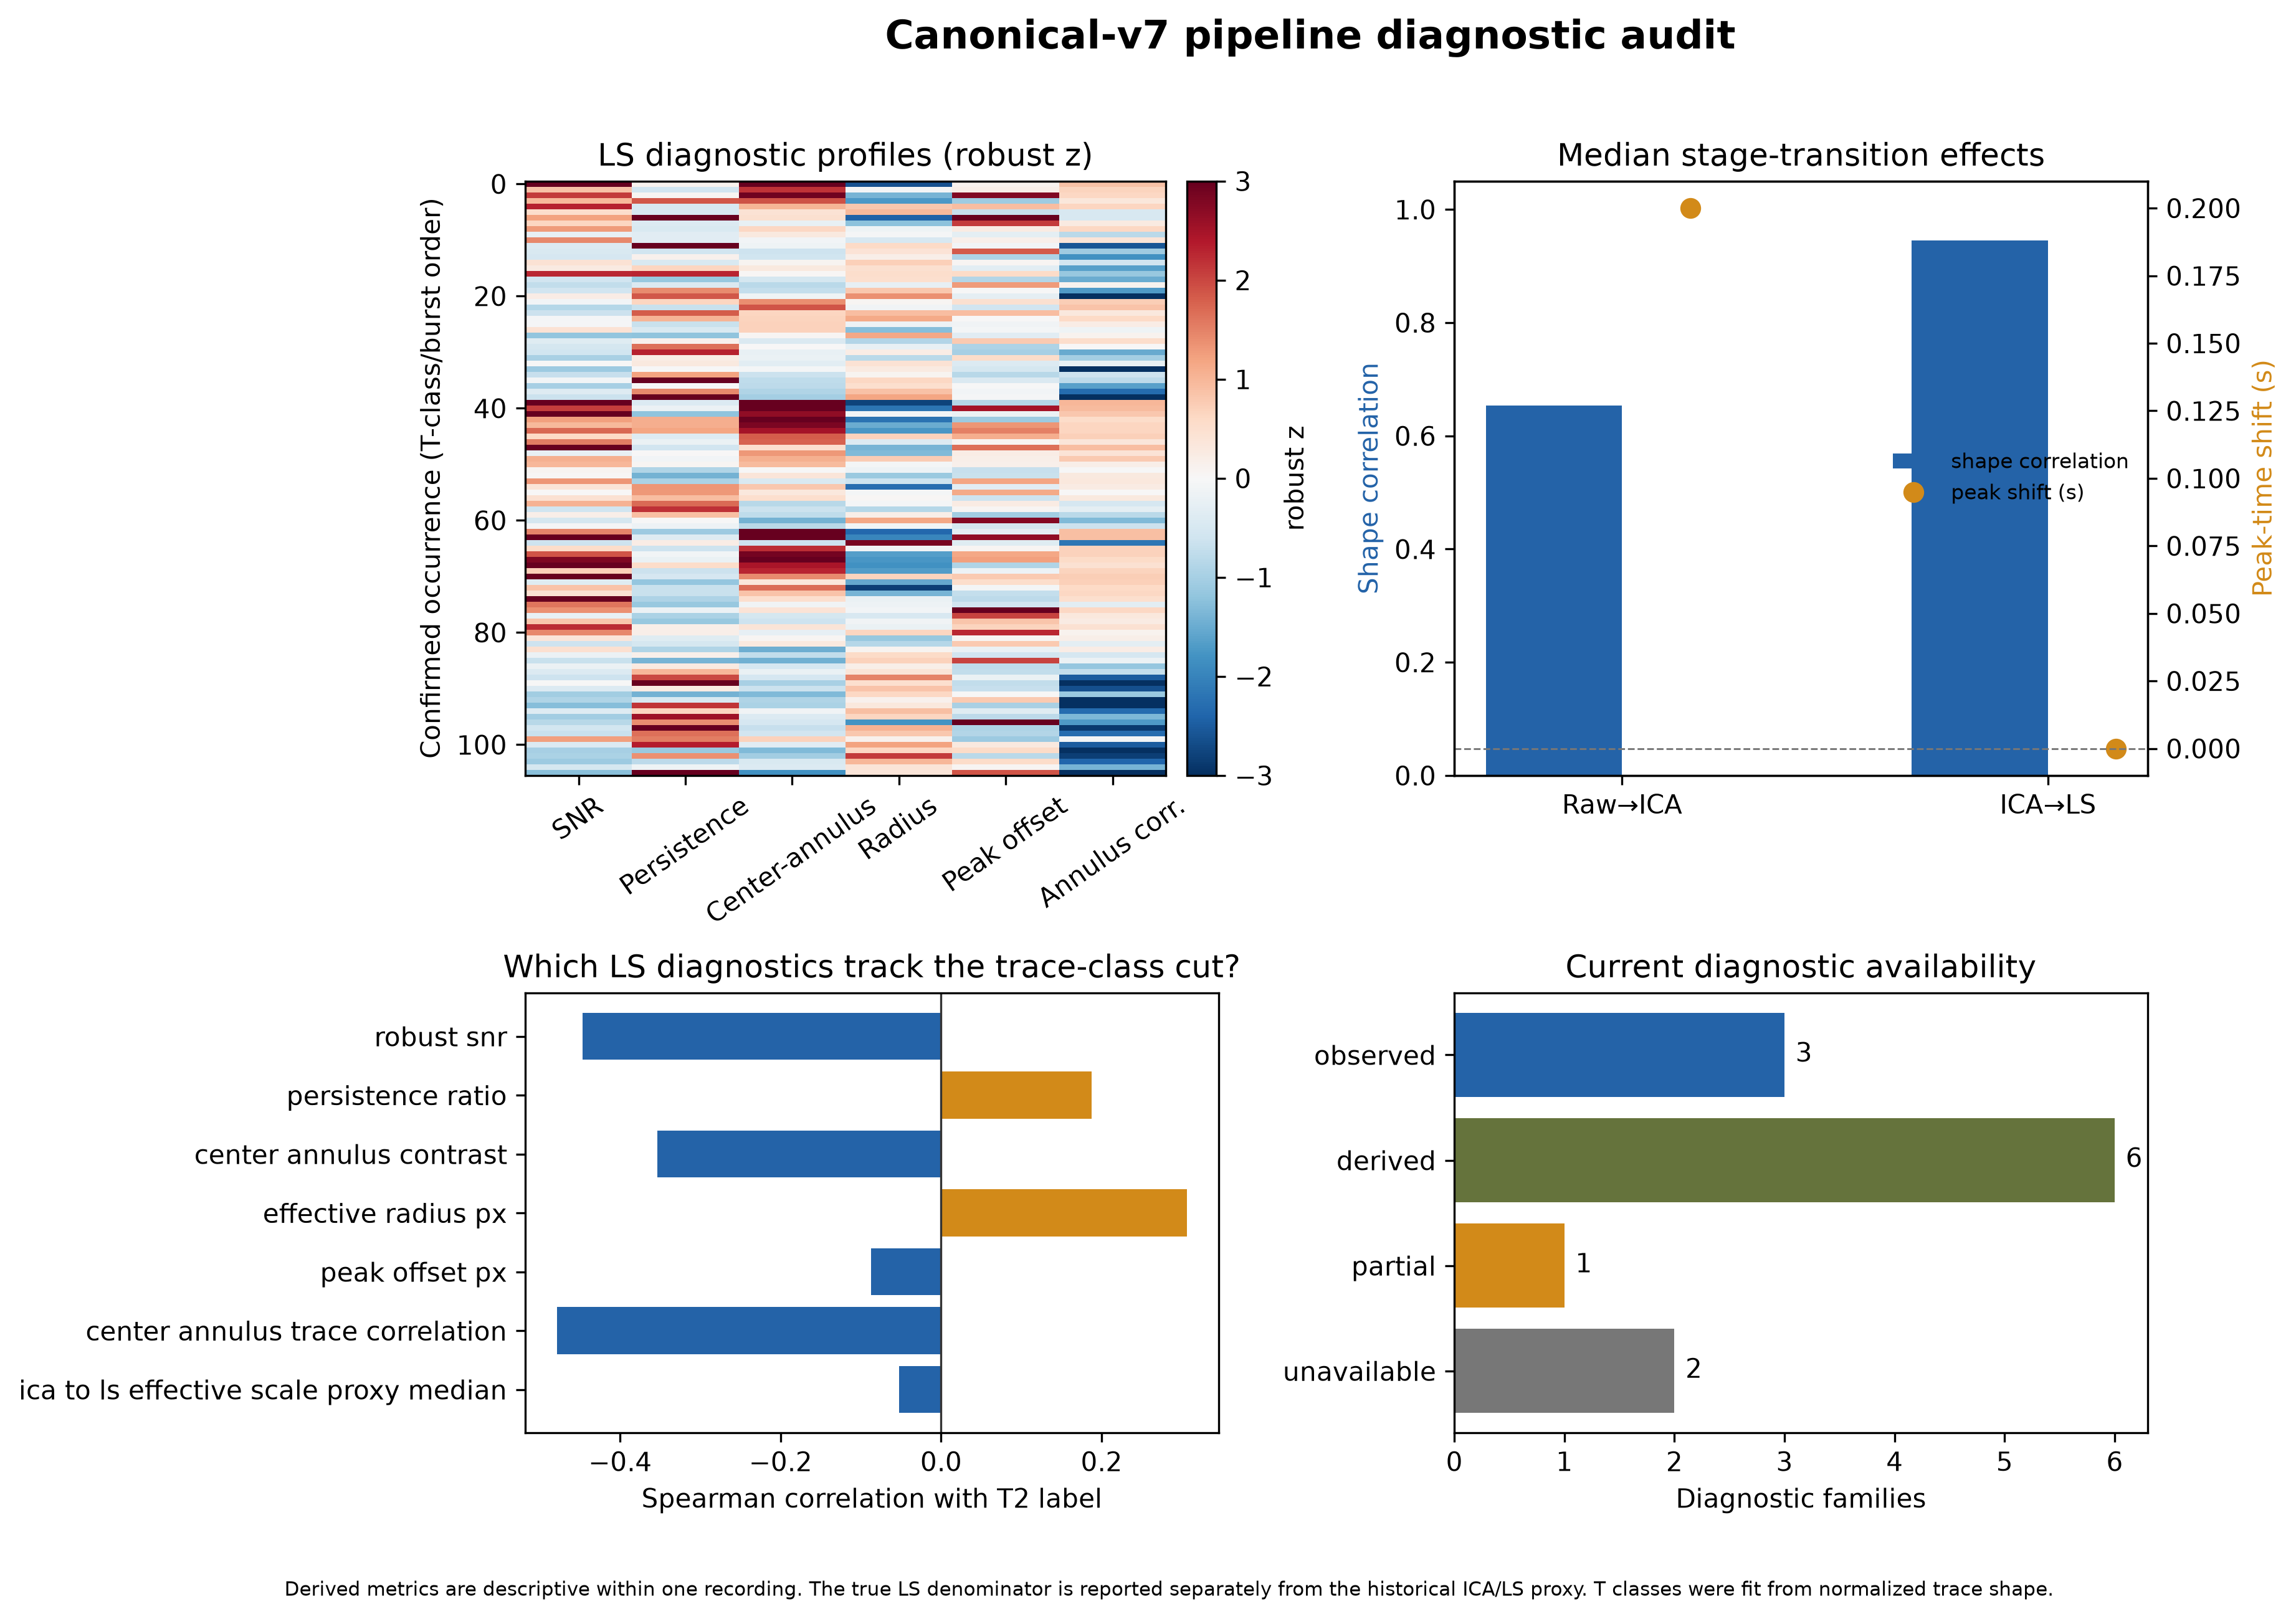
\includegraphics[width=0.98\linewidth]{figures/final/fig05_pipeline_diagnostic_audit.png}
  \caption{Current pipeline diagnostic audit. The availability panel now
  includes component-level ICA and true local-standardization denominator
  diagnostics; motion residuals and independent validation remain missing.}
  \label{fig:overview-audit}
\end{figure}

\subsection{The complete trace assigns features to different jobs}

The full-trace panel asks whether the annotated burst is exceptional relative
to every same-duration guarded quiet window at the same confirmed center
(\Cref{fig:overview-full-trace}). The carrier mean percentile is
\FullTraceCarrierPercentile{}, and \FullTraceCarrierCeilingCount{} of
\FullTraceOccurrences{} occurrence scores are exactly 1.0. Local coherence and
lagged recurrence are similarly saturated and do not beat the carrier under the
prespecified paired interval gate. This does not undo the earlier result that
coherence improves full-field known-positive recovery at a scarce candidate
budget. Instead, it separates feature roles: amplitude is enough once the
correct center is known; spatial coherence helps find or rank that center.

The two new summaries---agreement across Raw, ICA, and local-standardization
representations, and persistence across 3-, 7-, and 15-frame scales---do not
improve localization. Their median cross-burst site-rank correlations are
\FullTraceConsensusRepeatability{} and
\FullTracePersistenceRepeatability{}, respectively, making them exploratory
site-reliability features for independent confirmation.

\begin{figure}[p]
  \centering
  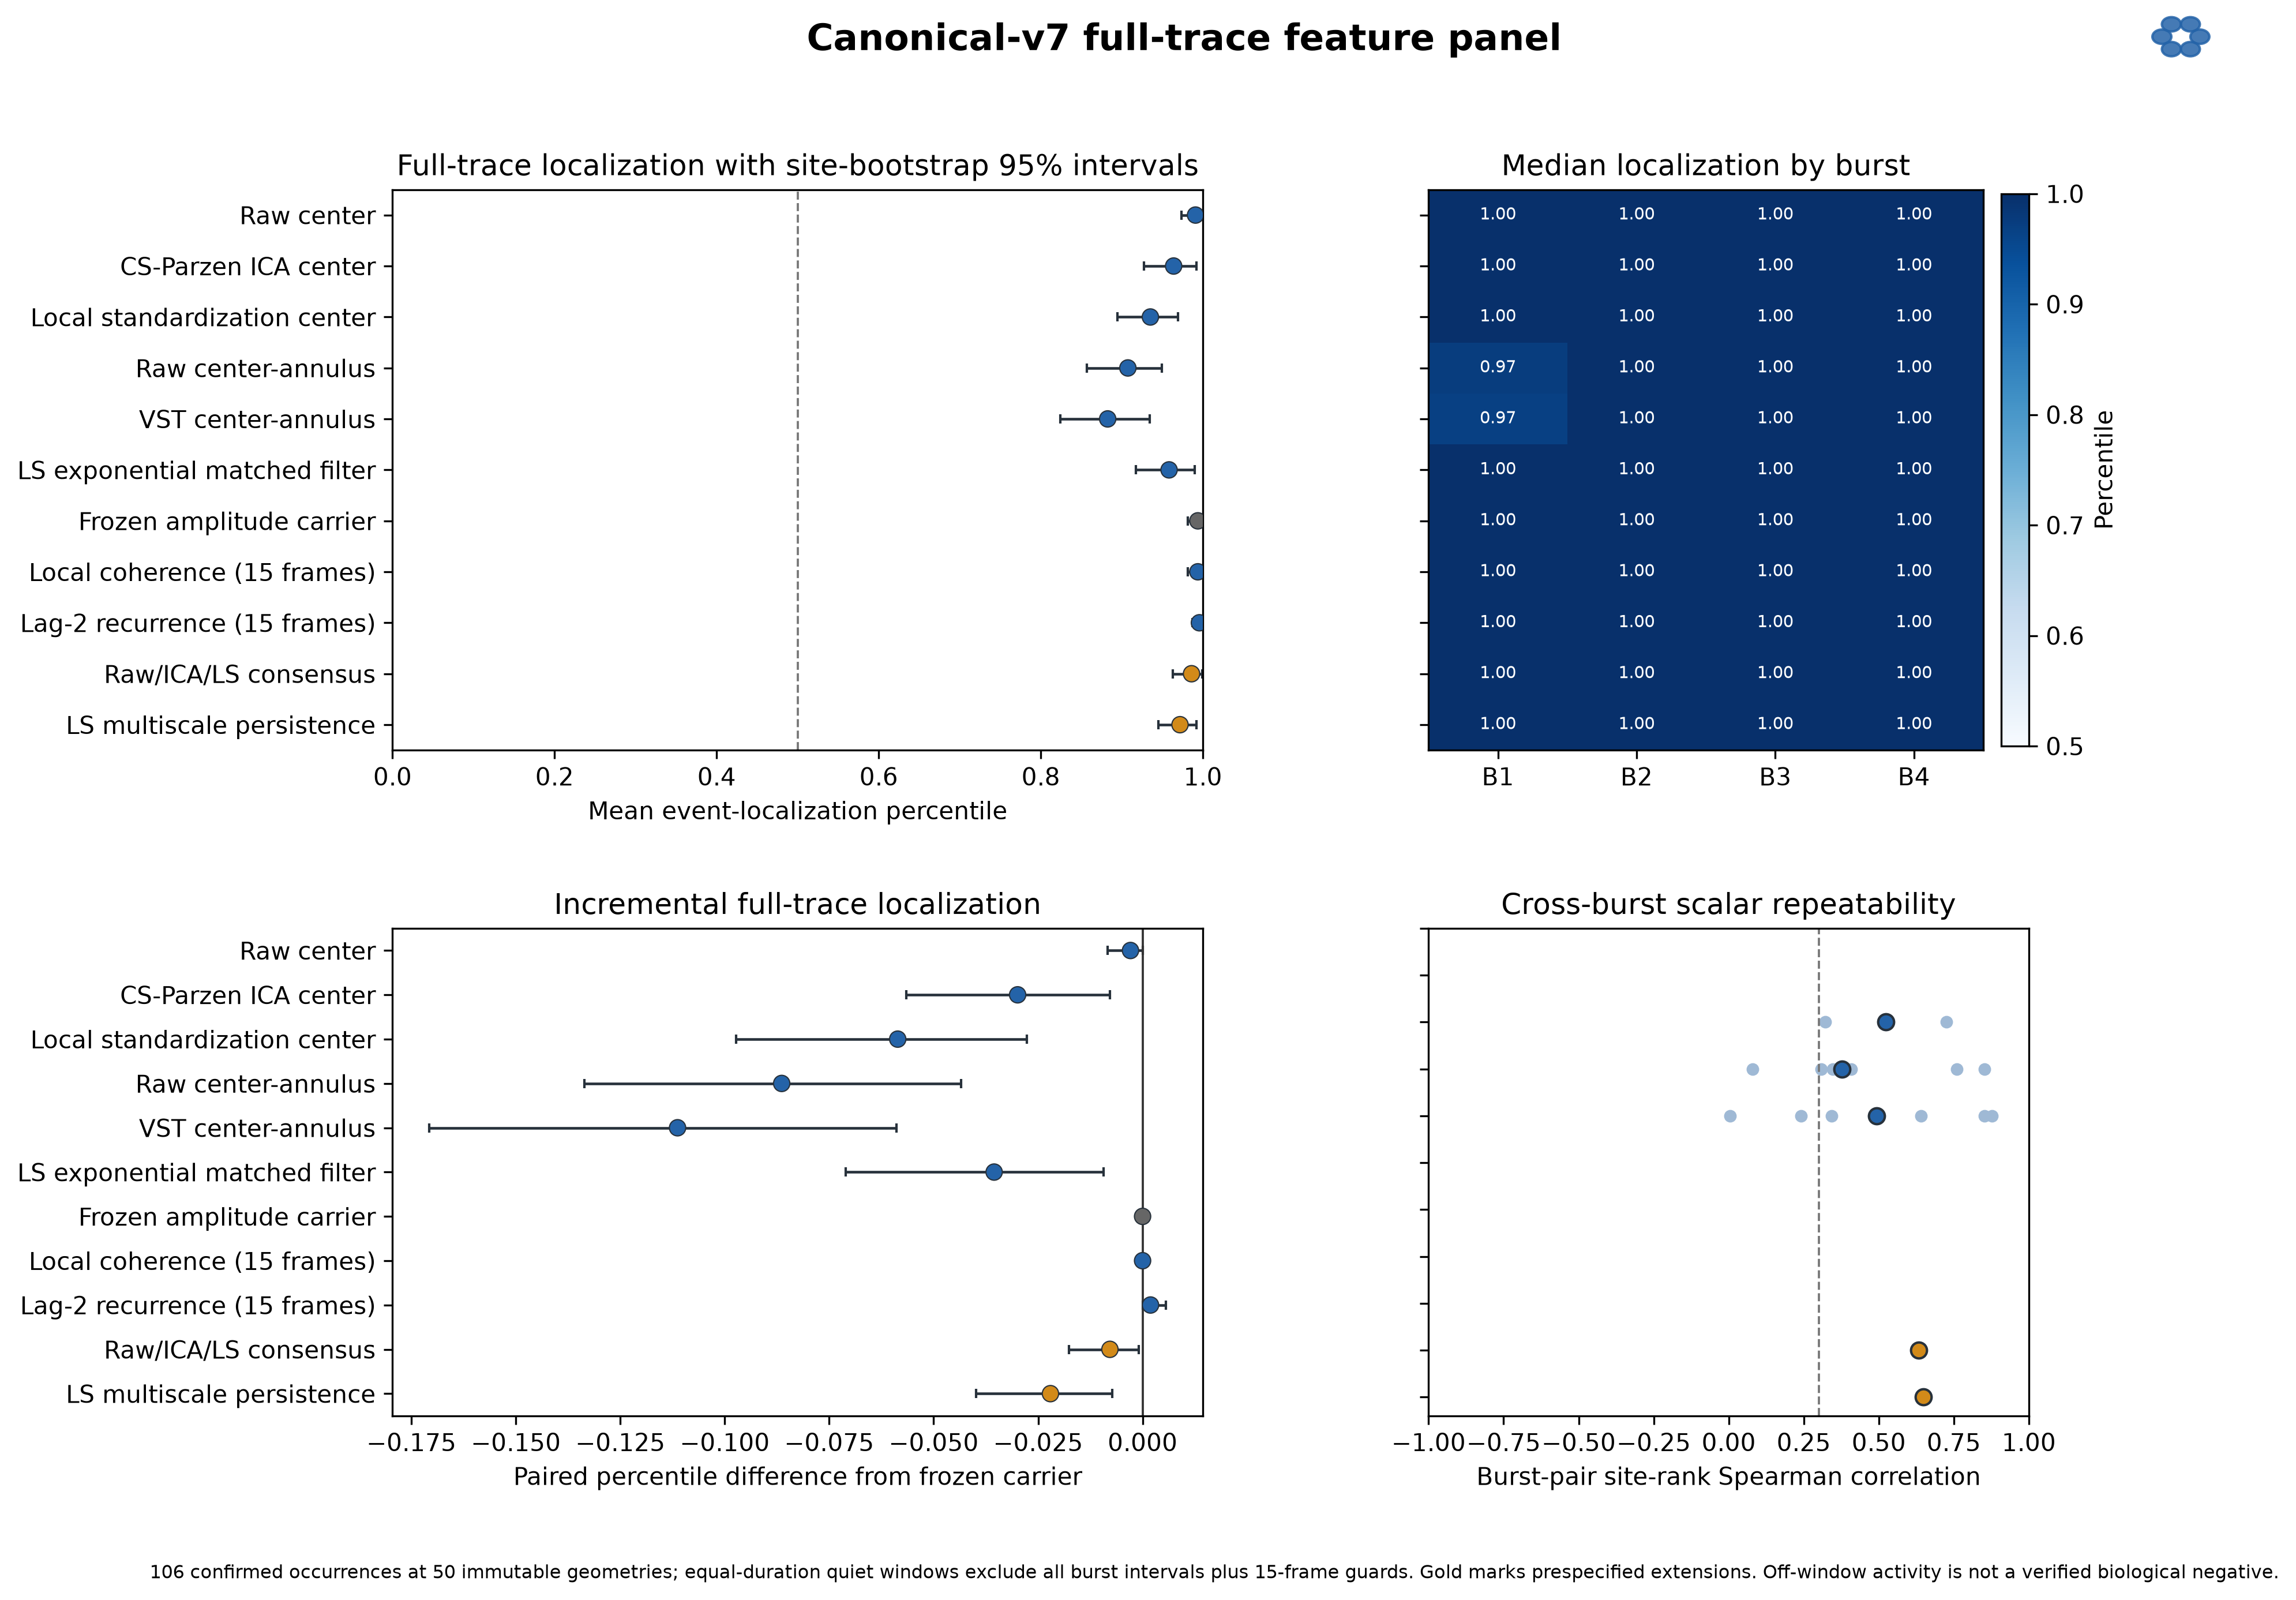
\includegraphics[width=0.98\linewidth]{figures/final/fig08_full_trace_feature_panel.png}
  \caption{Complete-trace feature panel at 50 confirmed sites. Quiet windows
  are temporal references rather than biological negatives. Gold denotes the
  two prespecified extensions.}
  \label{fig:overview-full-trace}
\end{figure}

\subsection{Automated challenge tests separate retrieval, localization, and reliability}

The ceiling-limited event-maximum result was followed by six fixed automated
tests (\Cref{fig:overview-automated}). In the harder frame-level retrieval task,
Raw led with AUC \AutoRawAUC{} [\AutoRawAUCLow{},
\AutoRawAUCHigh{}], followed by the carrier, coherence, and lag recurrence.
All six compact features were stronger at the labeled center than at
same-field, quiet-baseline-matched displaced tissue. The recovery target was
met by \AutoRecoveryCount{}/\FullTraceOccurrences{} original geometries.
Cross-fitted log loss improved from \AutoCarrierLogLoss{} to
\AutoExtendedLogLoss{} with the role-specific panel, but the site-bootstrap
improvement interval (\AutoRecoveryDeltaLow{}--\AutoRecoveryDeltaHigh{}) crossed
zero. Feature complementarity is therefore promising, not confirmed.

Coordinate and timing perturbations, 500 site-blocked circular shifts, and
fixed synthetic transients further distinguish robustness from biological
validity (\Cref{fig:overview-robustness}). The strongest amplitude/context
features degraded gradually under coordinate error and small timing shifts.
Every observed selected-feature alignment exceeded the circular-shift null,
while a calcium-shaped matched filter had the strongest weak-transient
injection response. These checks validate operator behavior; they do not create
ground-truth neurons or verified negative tissue.

\begin{figure}[p]
  \centering
  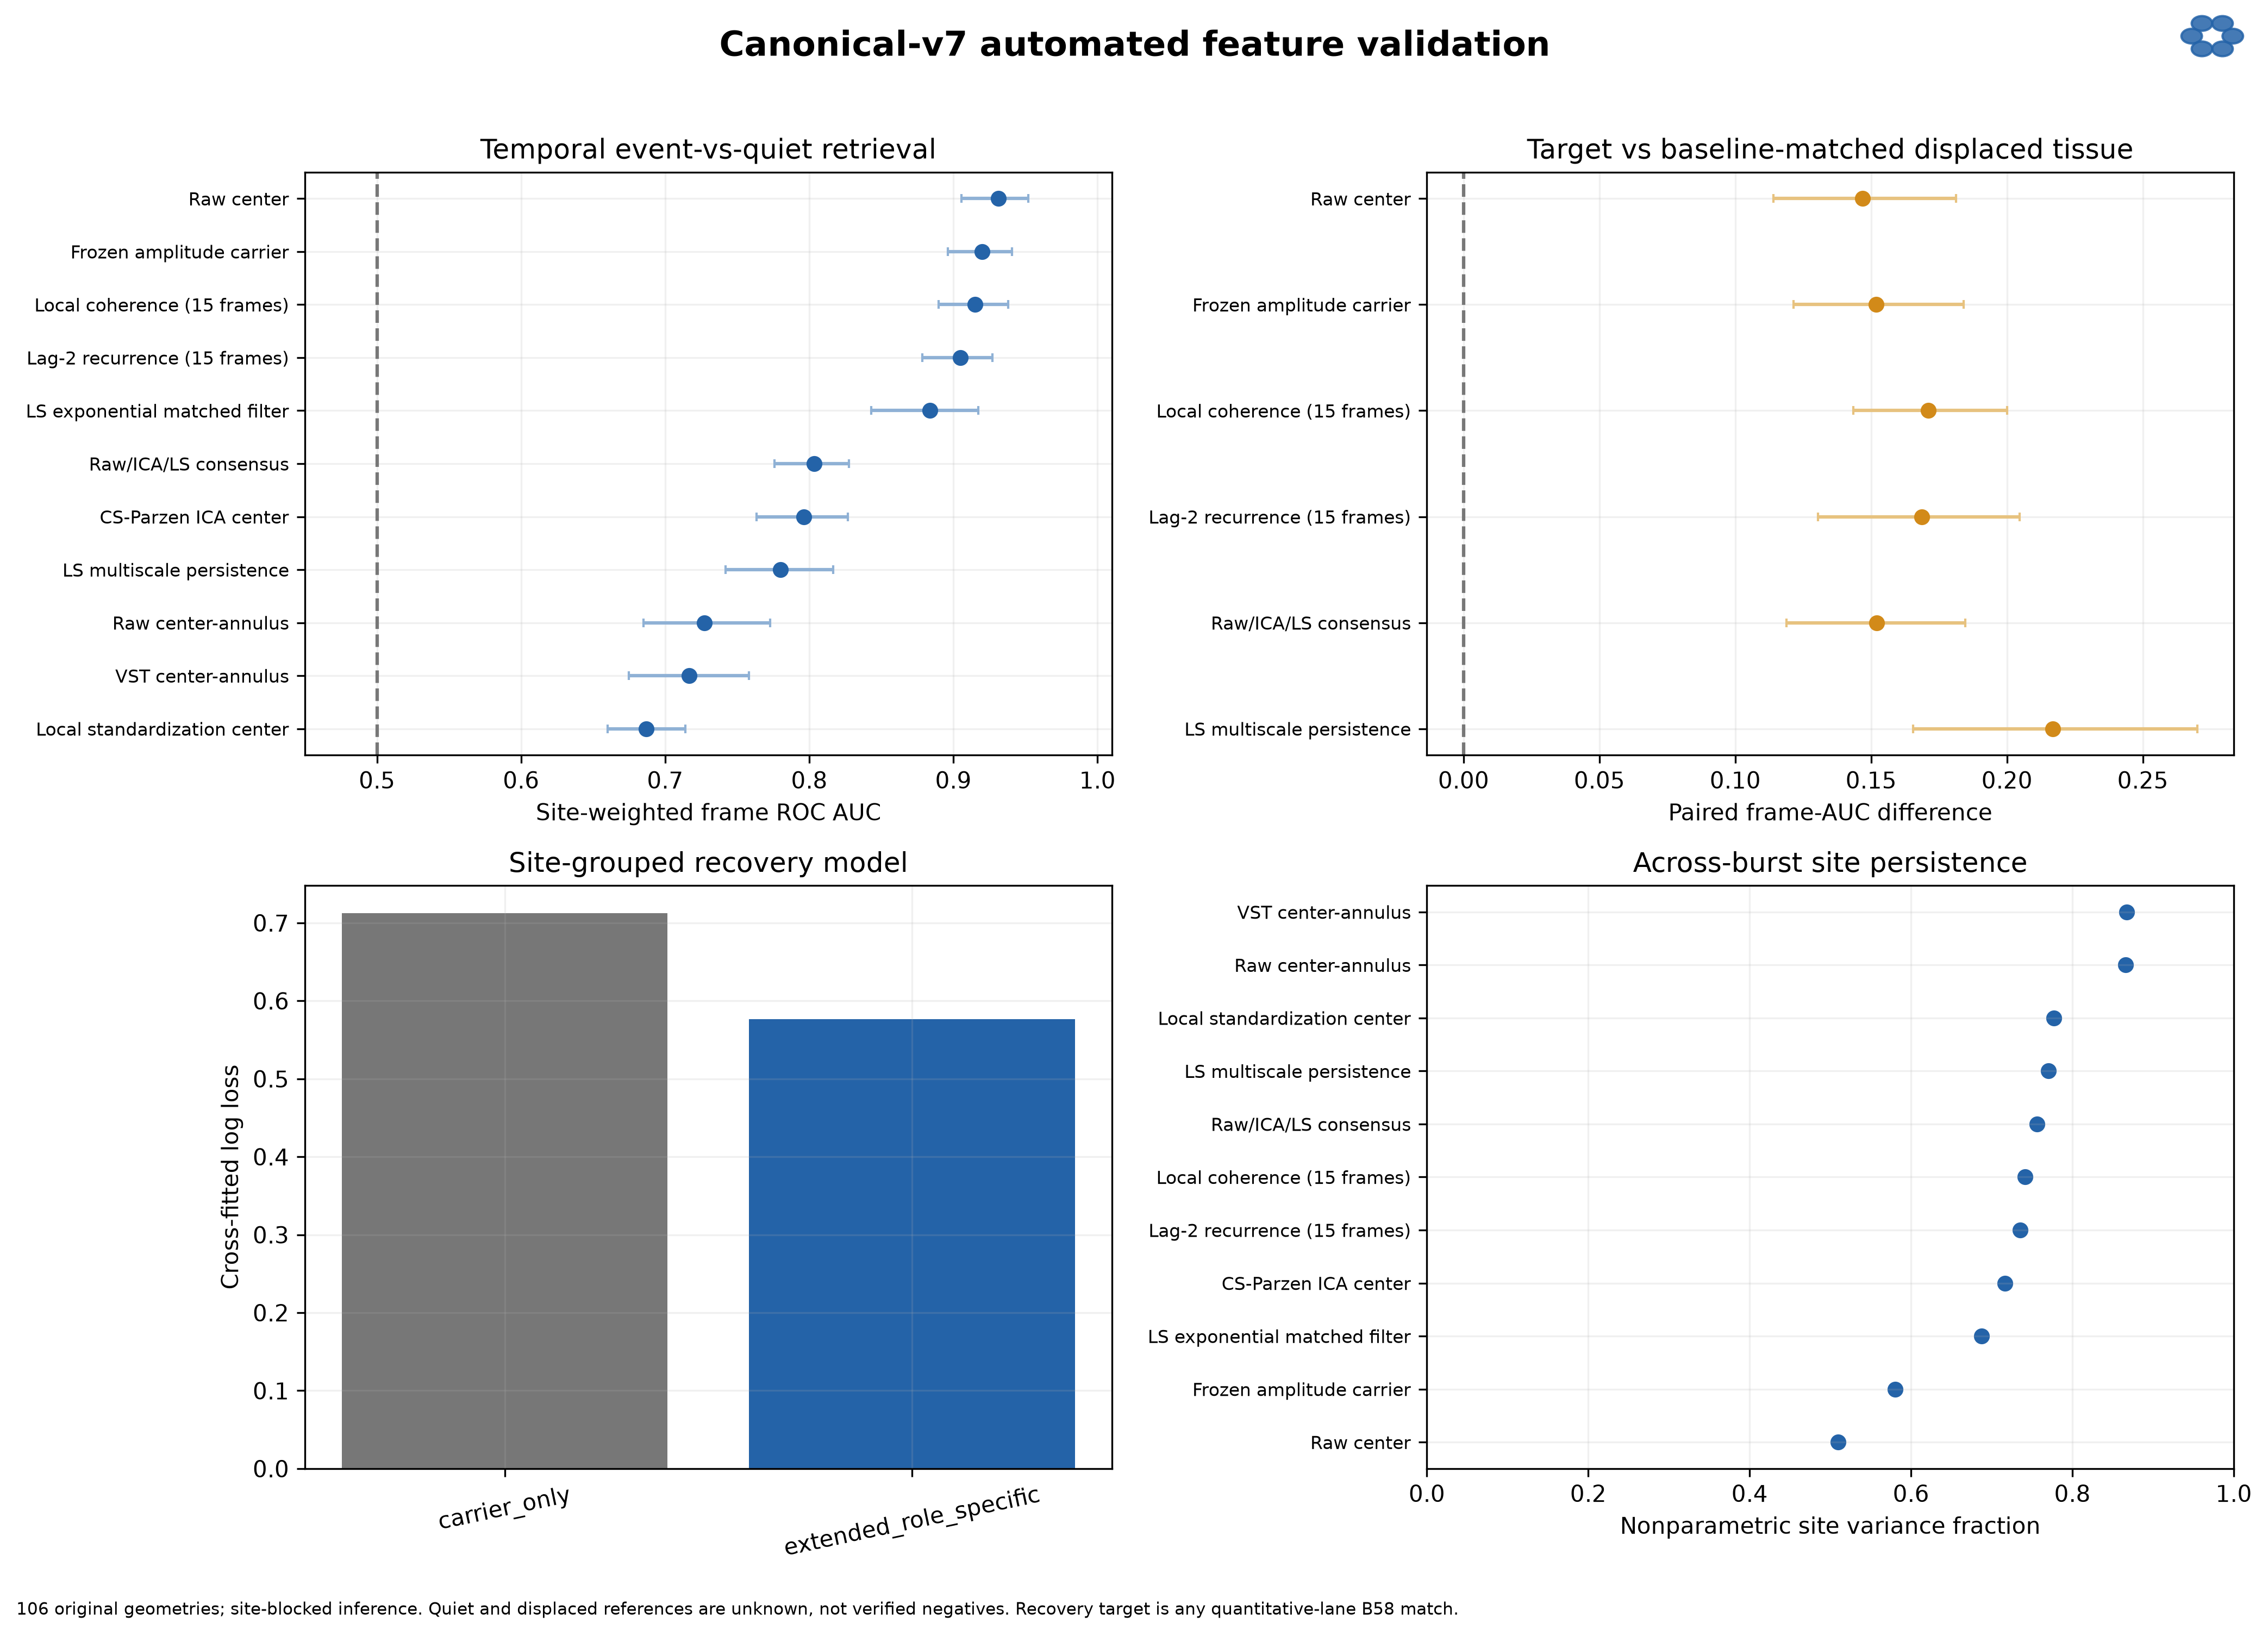
\includegraphics[width=0.98\linewidth]{figures/final/fig09_automated_feature_validation.png}
  \caption{Automated feature challenge suite. Site-blocked intervals preserve
  immutable geometry. Quiet and displaced references have unknown biological
  labels, and the recovery model remains exploratory.}
  \label{fig:overview-automated}
\end{figure}

\begin{figure}[p]
  \centering
  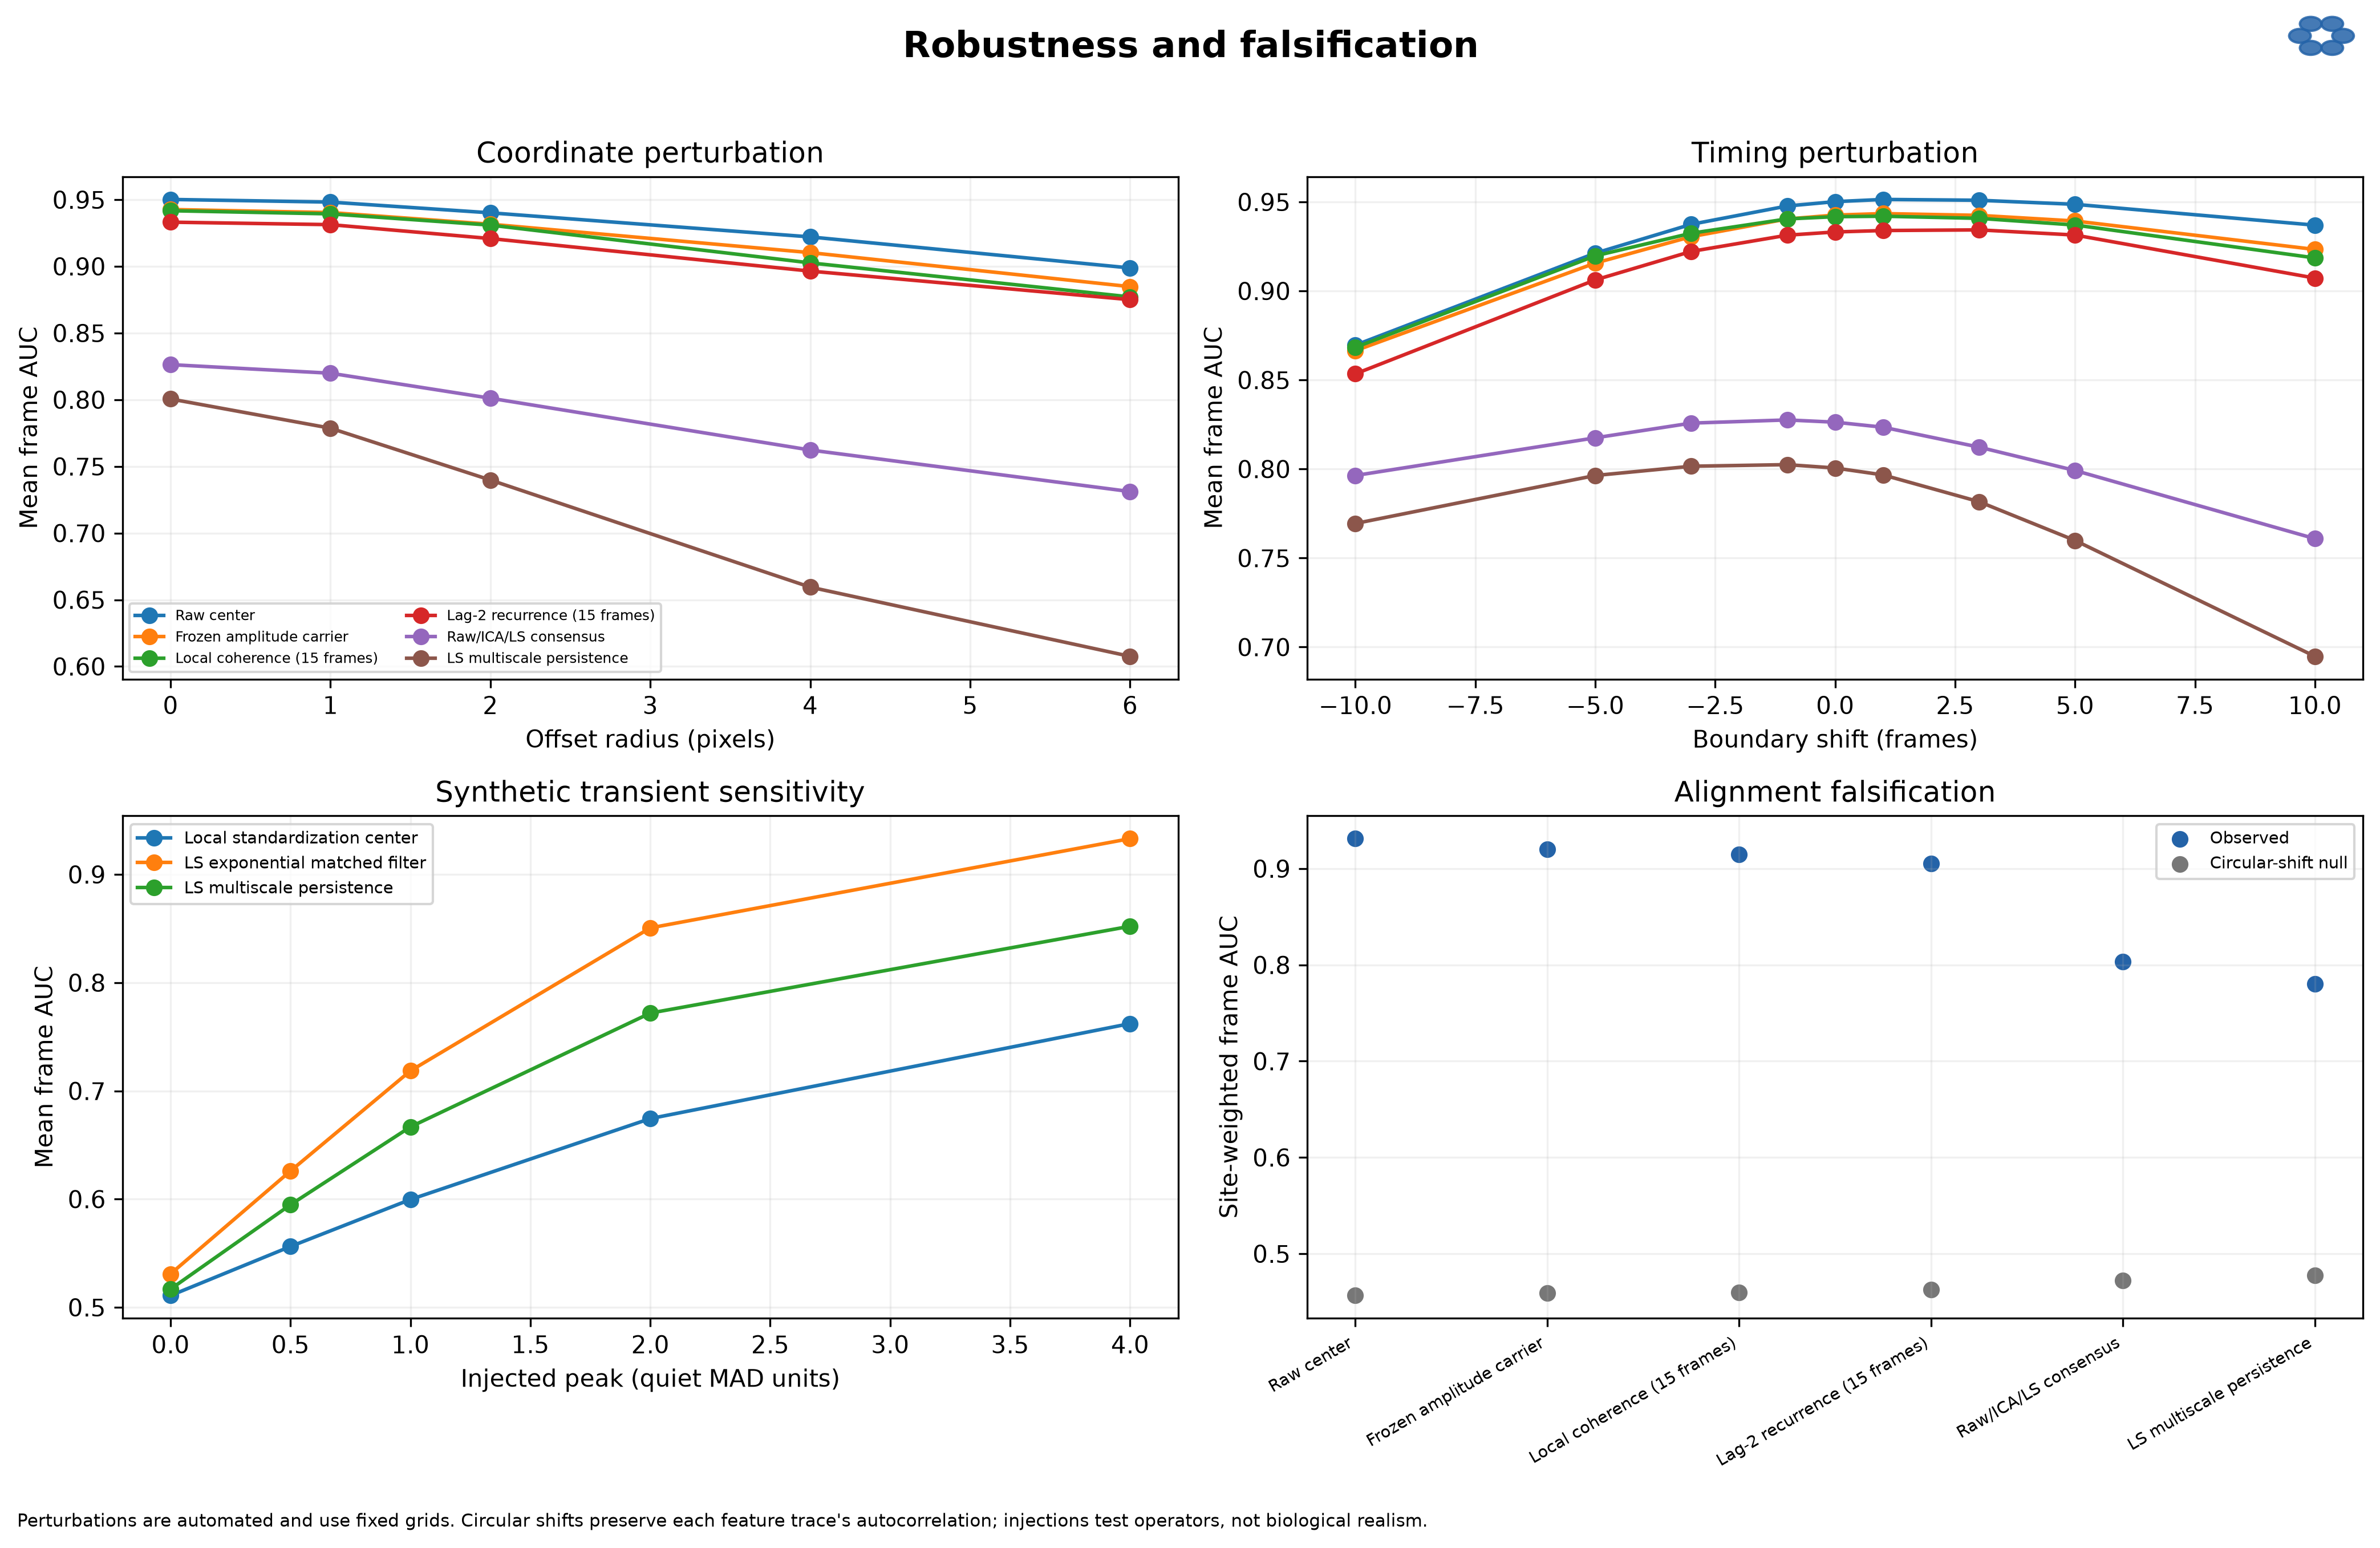
\includegraphics[width=0.98\linewidth]{figures/final/fig10_robustness_falsification.png}
  \caption{Coordinate and timing perturbations, synthetic transient
  sensitivity, and circular-shift alignment falsification. Injections test
  operators rather than realistic tissue or optical formation.}
  \label{fig:overview-robustness}
\end{figure}

The feature deep dives further separated pipeline roles. At B58,
\DeepRecoveredAll{} occurrences were recovered by all lanes,
\DeepRecoveredPartial{} by a subset, and \DeepAllMisses{} by none. At B20,
coherence and lag had native recall gains of \DeepCoherenceNativeTwenty{} and
\DeepLagNativeTwenty{} over carrier, compared with only
\DeepCoherenceRankingTwenty{} and \DeepLagRankingTwenty{} on a common proposal
universe. The selected kinetic kernel was \DeepKineticKernel{} with
leave-one-burst-out mean AUC \DeepKineticLOBOAUC{}. These results support
separate proposal, ranking, and kinetic roles while remaining within-recording
and exploratory.

The canonical-v8 review adds an identity guard to this failure interpretation.
Of the 12 all-lane misses, two local response maxima collided with another
geometry of the same canonical identity, six approached a different identity,
and four were identity-clear. Strict recall remains $94/106=88.7\%$; the
$94/98=95.9\%$ identity-resolved value is conditional and must not replace it.
The four-case rescue ceiling is $98/106=92.5\%$, contingent on independent
validation of ROI~19, ROI~22, ROI~25, and ROI~27.

\begin{table}[!htbp]
\centering
\caption{Canonical-v8 identity-aware interpretation of the frozen B58 recovery
result. Only strict recall is an official detector metric. Audit-conditioned
and hypothetical values are sensitivities, not replacement performance
estimates.}
\label{tab:identity-aware-v8}
\small
\begin{tabularx}{\linewidth}{>{\raggedright\arraybackslash}p{0.31\linewidth} >{\raggedright\arraybackslash}p{0.20\linewidth} X}
\toprule
Quantity & Value & Interpretation \\
\midrule
Strict recovered occurrences & $94/106=88.7\%$ & Frozen official known-positive recall; unchanged by v8. \\
Canonical-collapsed sensitivity & $93/102=91.2\%$ & Existing duplicate-collapsed sensitivity; unchanged by v8. \\
All-lane misses & $12/106=11.3\%$ & Frozen miss count entering the identity-aware audit. \\
Same-identity collisions & $2/12=16.7\%$ & Candidate approaches another geometry assigned to the same canonical identity. \\
Different-identity collisions & $6/12=50.0\%$ & Candidate approaches a different labeled canonical identity. \\
Identity-clear hypotheses & $4/12=33.3\%$ & ROI 19, 22, 25, and 27 remain unresolved localization, noise, ranking, or NMS hypotheses. \\
Identity-resolved conditional sensitivity & $94/98=95.9\%$ & Descriptive sensitivity after excluding eight collision occurrences from the evaluable denominator; not official recall. \\
Four-case rescue ceiling & $98/106=92.5\%$ & Hypothetical strict recall if every identity-clear candidate were independently validated and recovered. \\
\bottomrule
\end{tabularx}
\end{table}


The automated follow-up supports the identity distinction. Collision cases had
more consistent shift directions across Raw, ICA, and local standardization
(median cosine 0.972 versus 0.448) and greater neighboring-trace leakage after
conditioning on the original center (median partial correlation 0.474 versus
0.182). Morphology alone separated the groups weakly. Response-weighted
footprints increased event SNR in both groups, showing that spatial aggregation
can improve visibility without proving that the aggregated signal belongs to
the intended identity (\Cref{fig:overview-identity-aware}).

\begin{figure}[p]
  \centering
  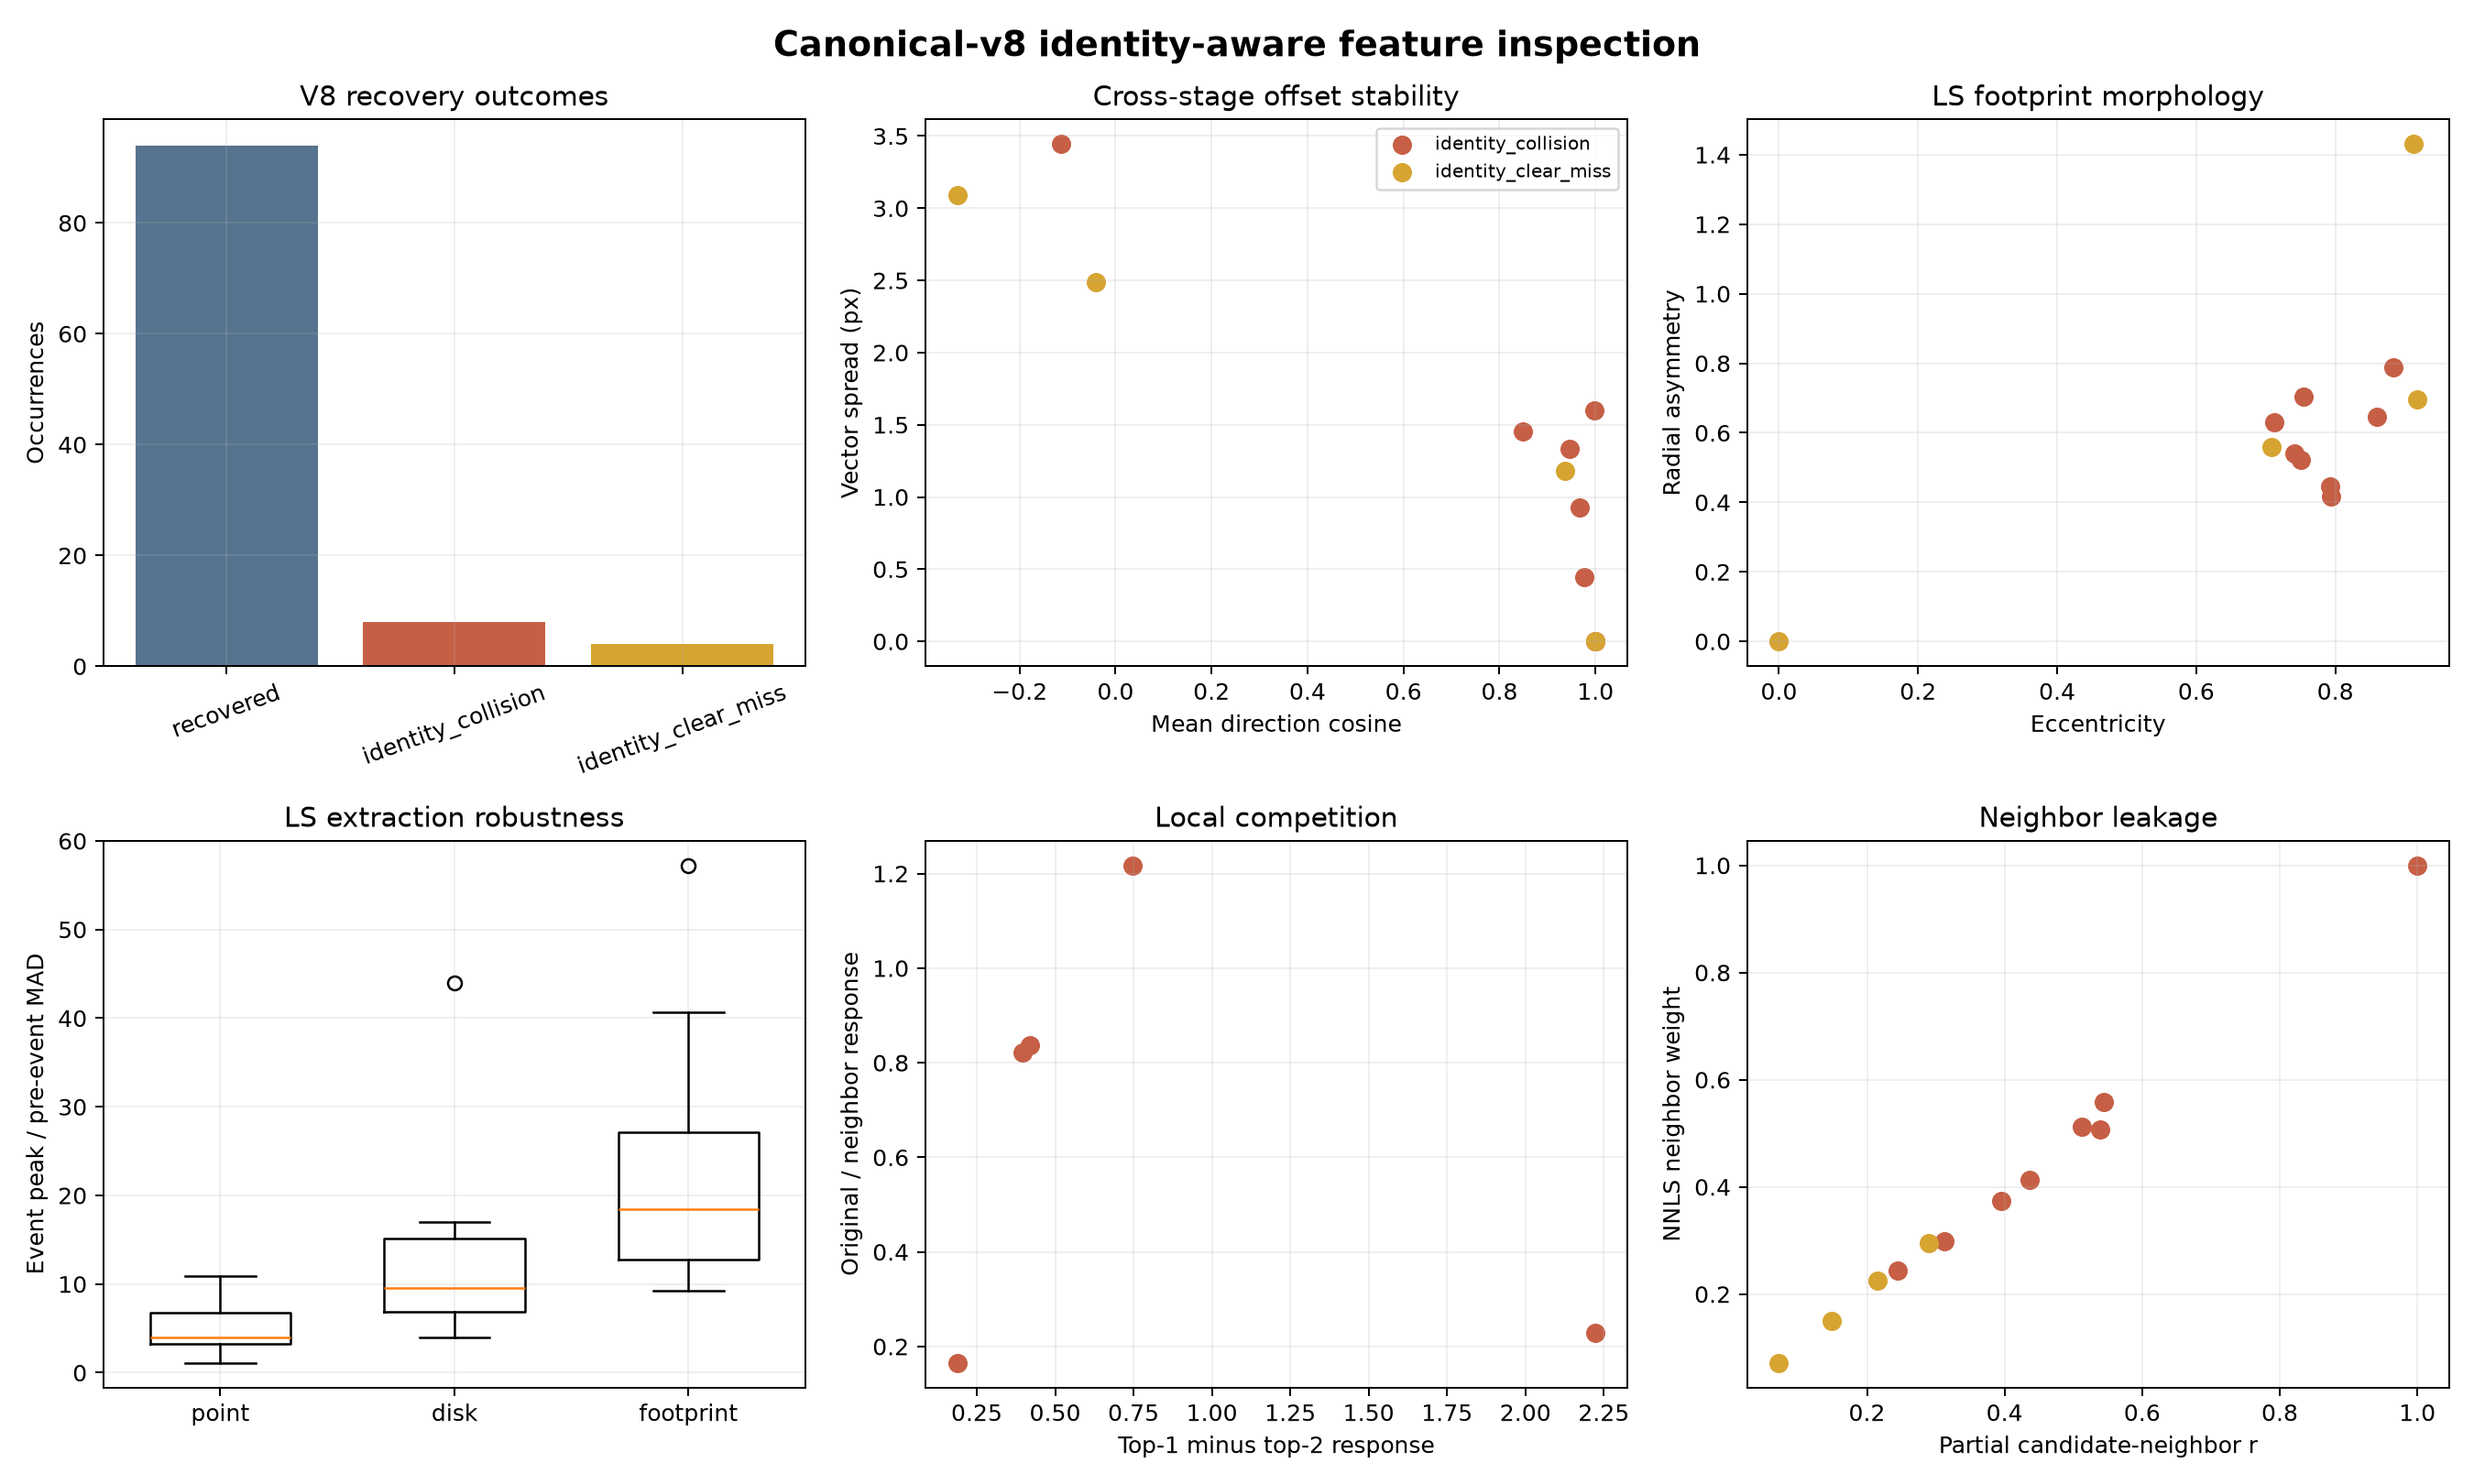
\includegraphics[width=0.99\linewidth]{figures/final/fig13_identity_aware_feature_inspection_v8.png}
  \caption{Identity-aware feature inspection of the 12 all-lane misses. The
  collision and identity-clear groups are descriptive and contain only eight
  and four occurrences.}
  \label{fig:overview-identity-aware}
\end{figure}

The expanded automated suite found that the full stack predicts frozen recovery
more effectively than carrier alone under identity grouping (AUC 0.833 versus
0.611). Variance-stabilized annular context and multiscale persistence were the
most stable sparse selections, followed by lag recurrence. This favors an
observability-context interpretation rather than brightness alone. Abstaining
on the least-confident half reduced internal error from 20.8\% to 9.4\%, while
recovered-only anomaly scoring reached AUC 0.814 for prioritizing misses. These
results remain internal and exploratory
(\Cref{fig:overview-expanded-validation}).

\begin{figure}[p]
  \centering
  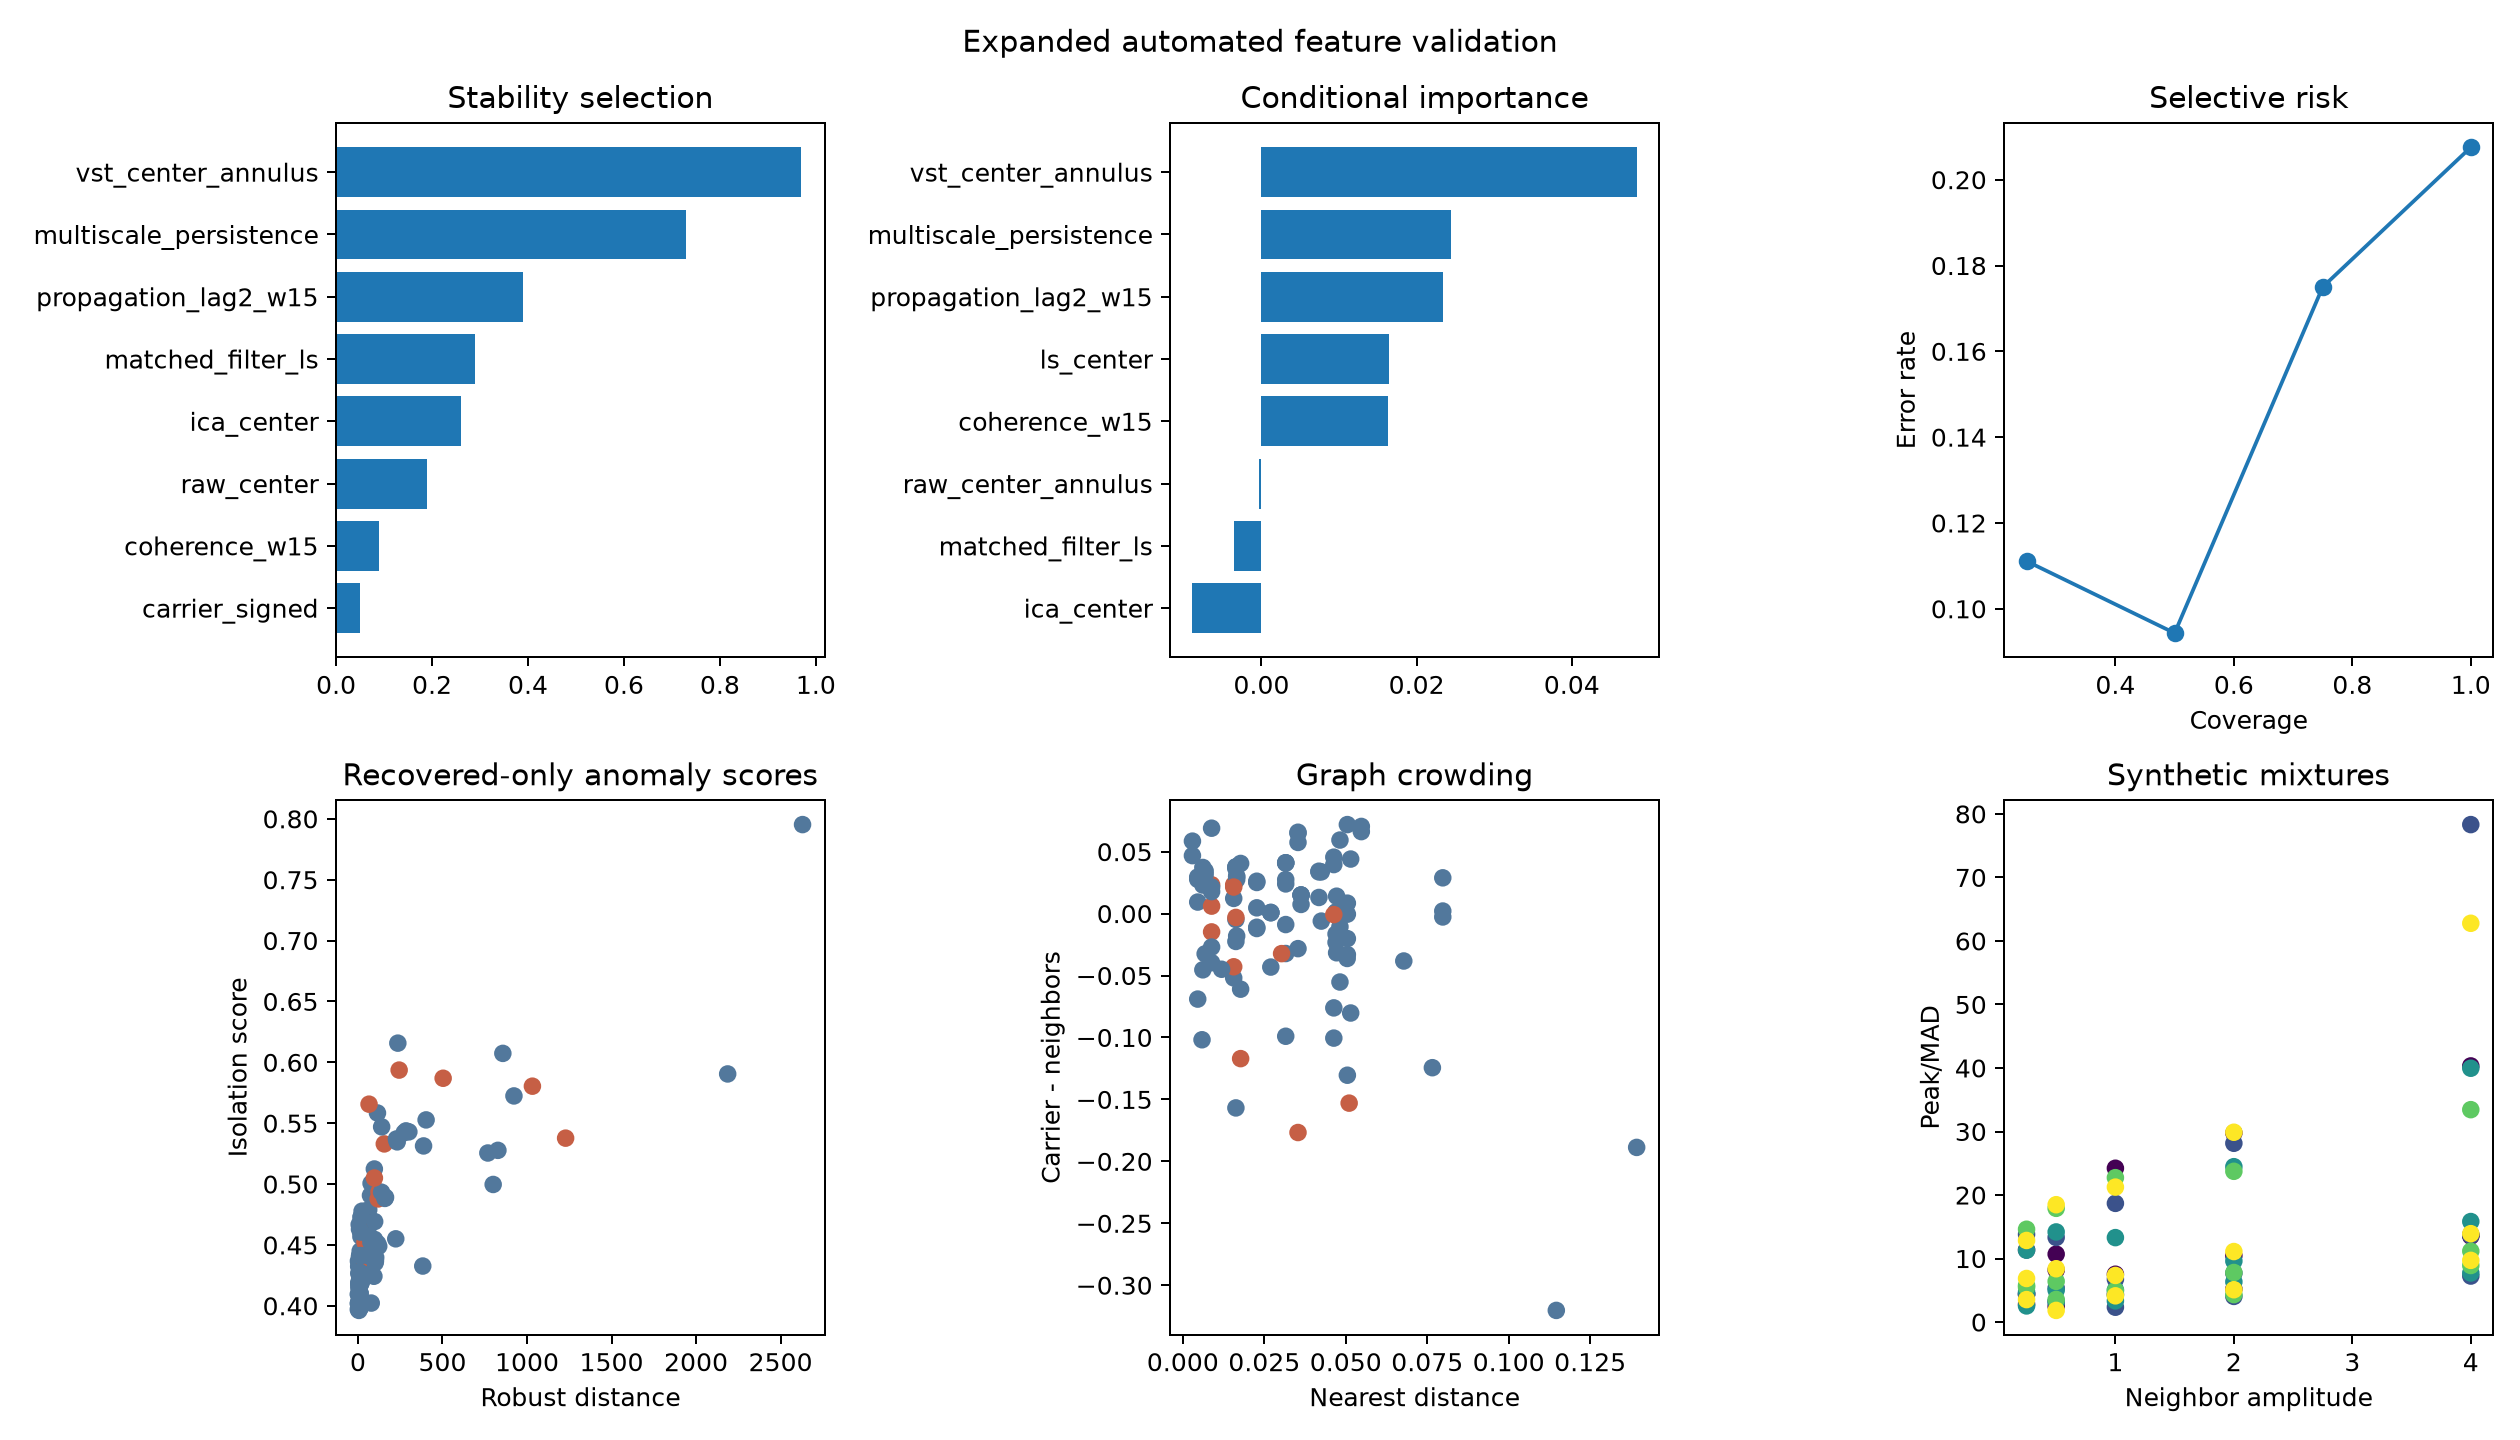
\includegraphics[width=0.99\linewidth]{figures/final/fig14_expanded_automated_validation.png}
  \caption{Expanded non-RL automated validation of feature stability,
  conditional importance, abstention, anomaly prioritization, graph context,
  and controlled mixtures.}
  \label{fig:overview-expanded-validation}
\end{figure}

\begin{figure}[p]
  \centering
  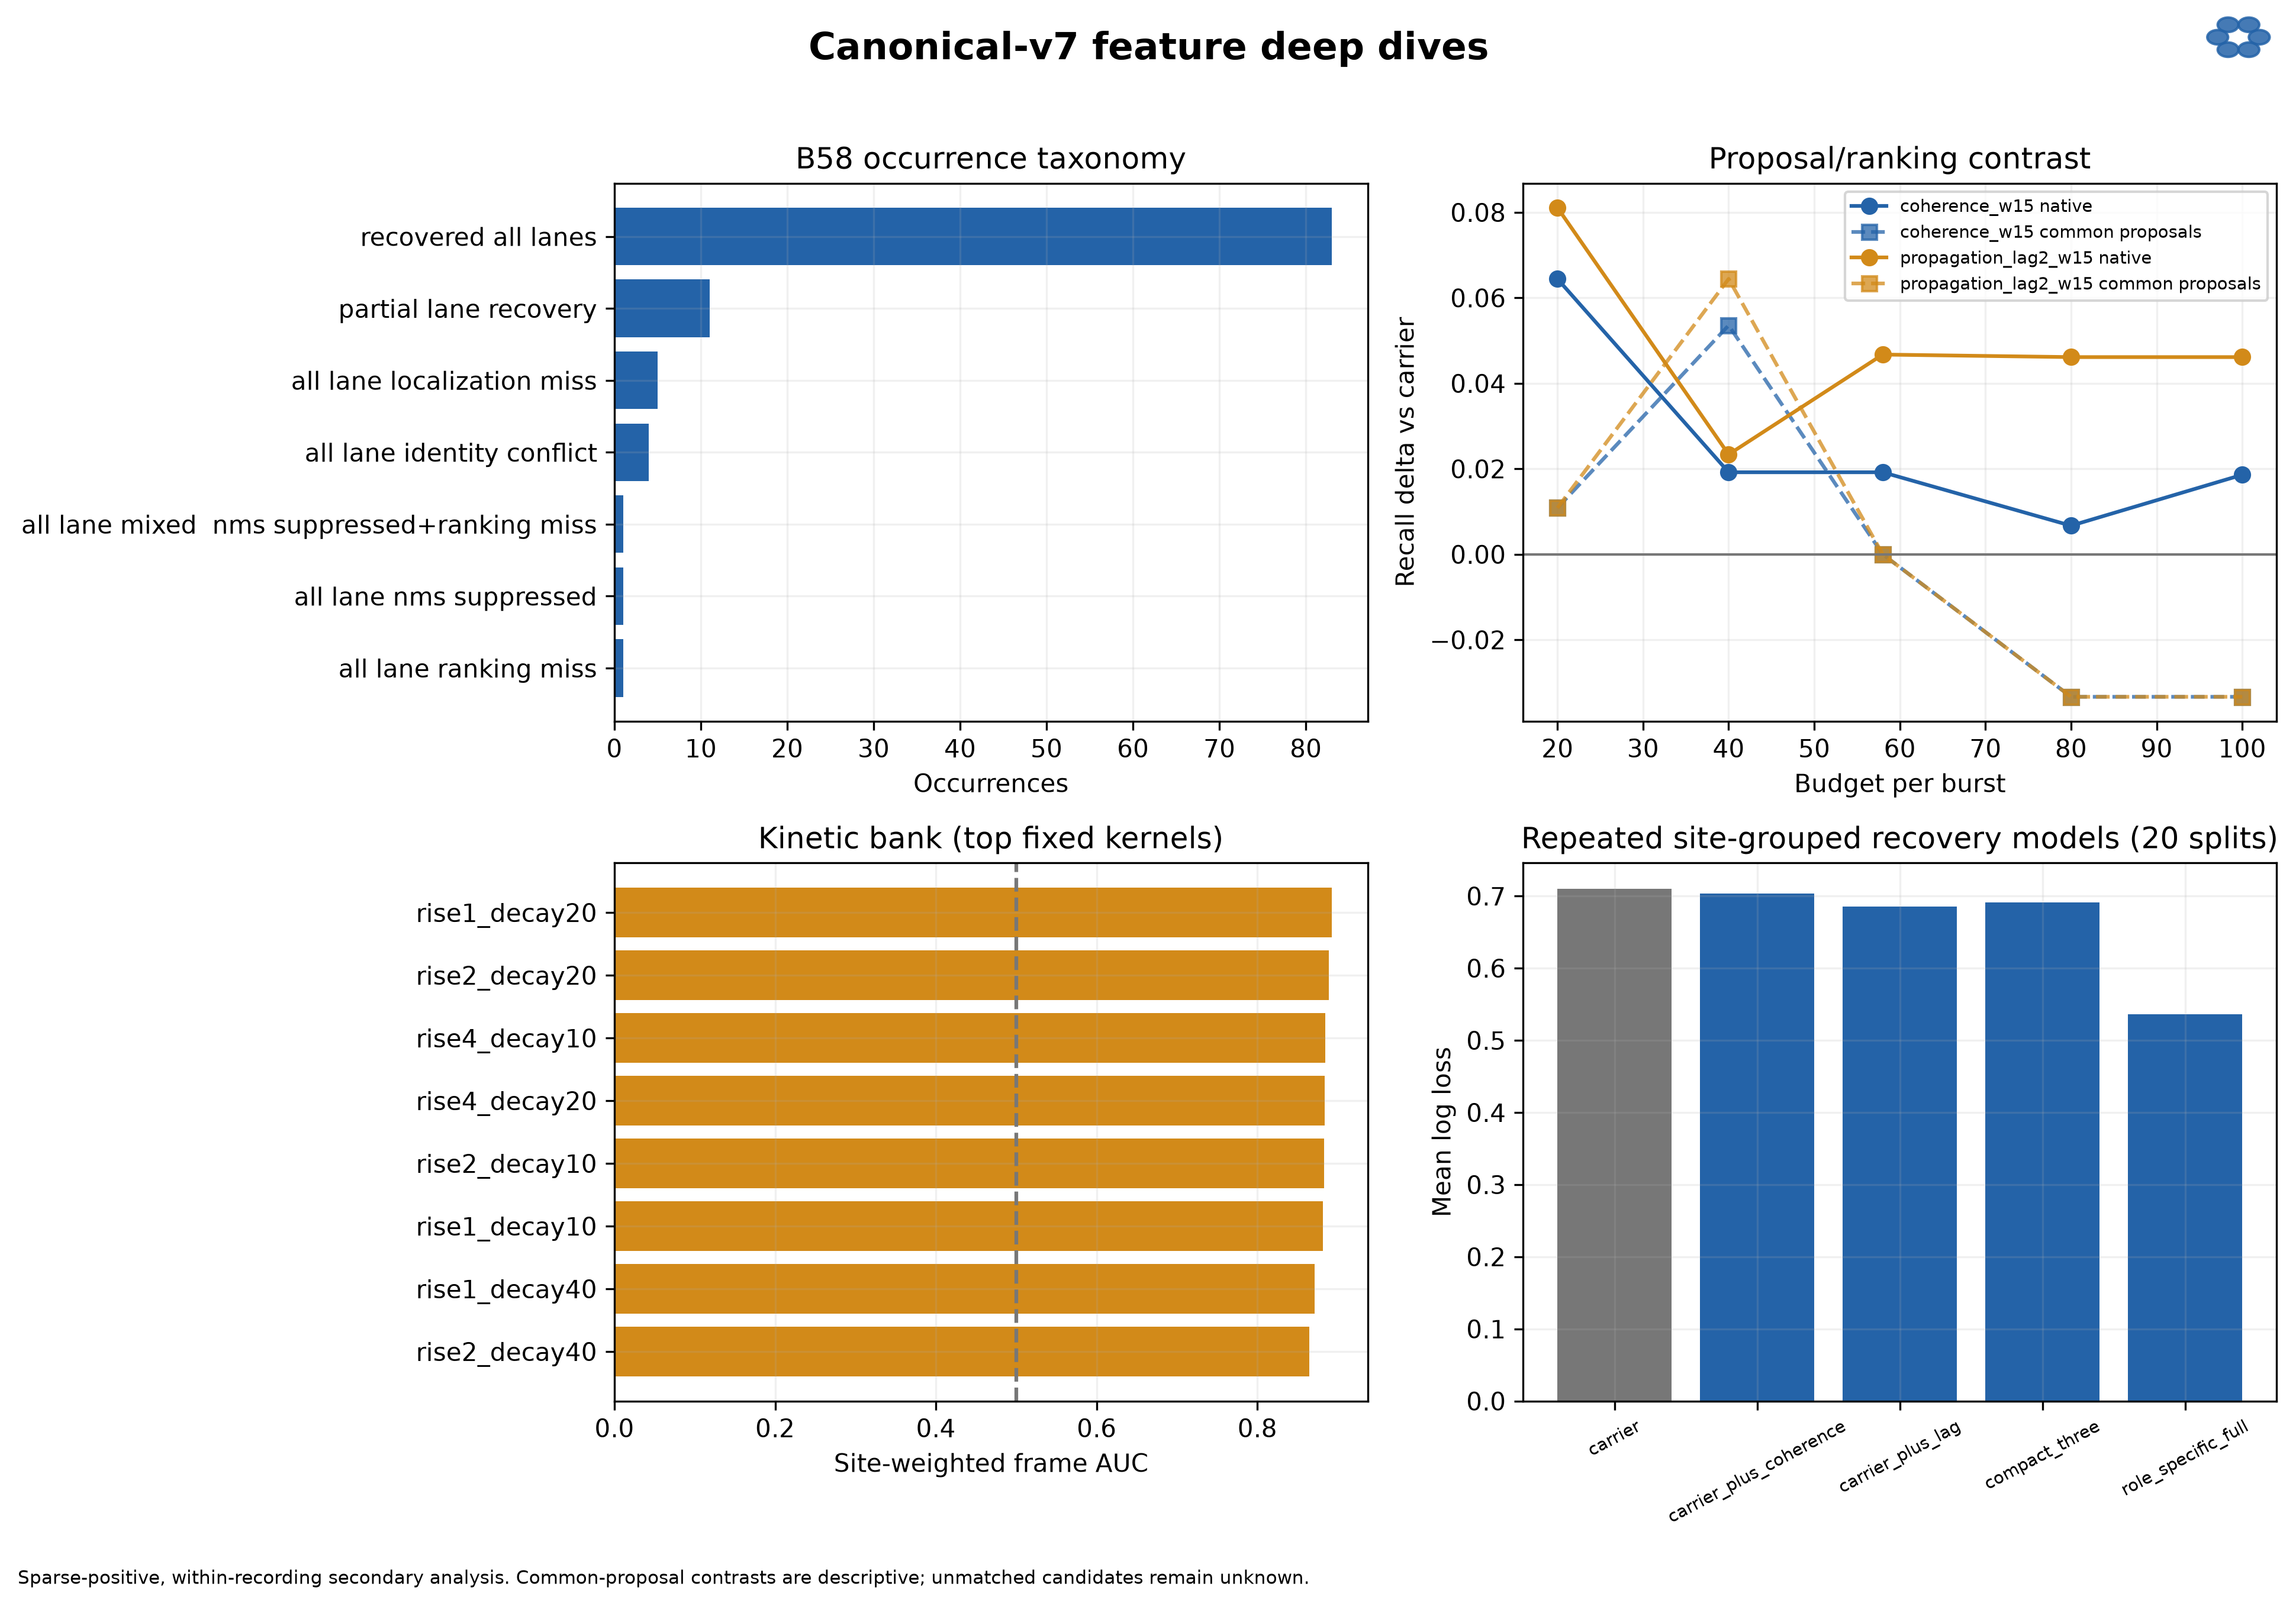
\includegraphics[width=0.98\linewidth]{figures/final/fig11_feature_deep_dives.png}
  \caption{Failure taxonomy, proposal/ranking contrasts, kinetic-bank results,
  and repeated grouped recovery models.}
  \label{fig:overview-feature-deep-dives}
\end{figure}

\subsection{What the model-internal diagnostics add}

The temporal transform is no longer a black box. All six component traces and
the fitted matrices are retained at each site (\Cref{fig:overview-ica}). The
maximum sitewise embedding inversion RMS is $5.69\times10^{-12}$. This confirms
that the fitted transform can be inverted numerically; it is not a denoising or
biological reconstruction score.

\begin{figure}[p]
  \centering
  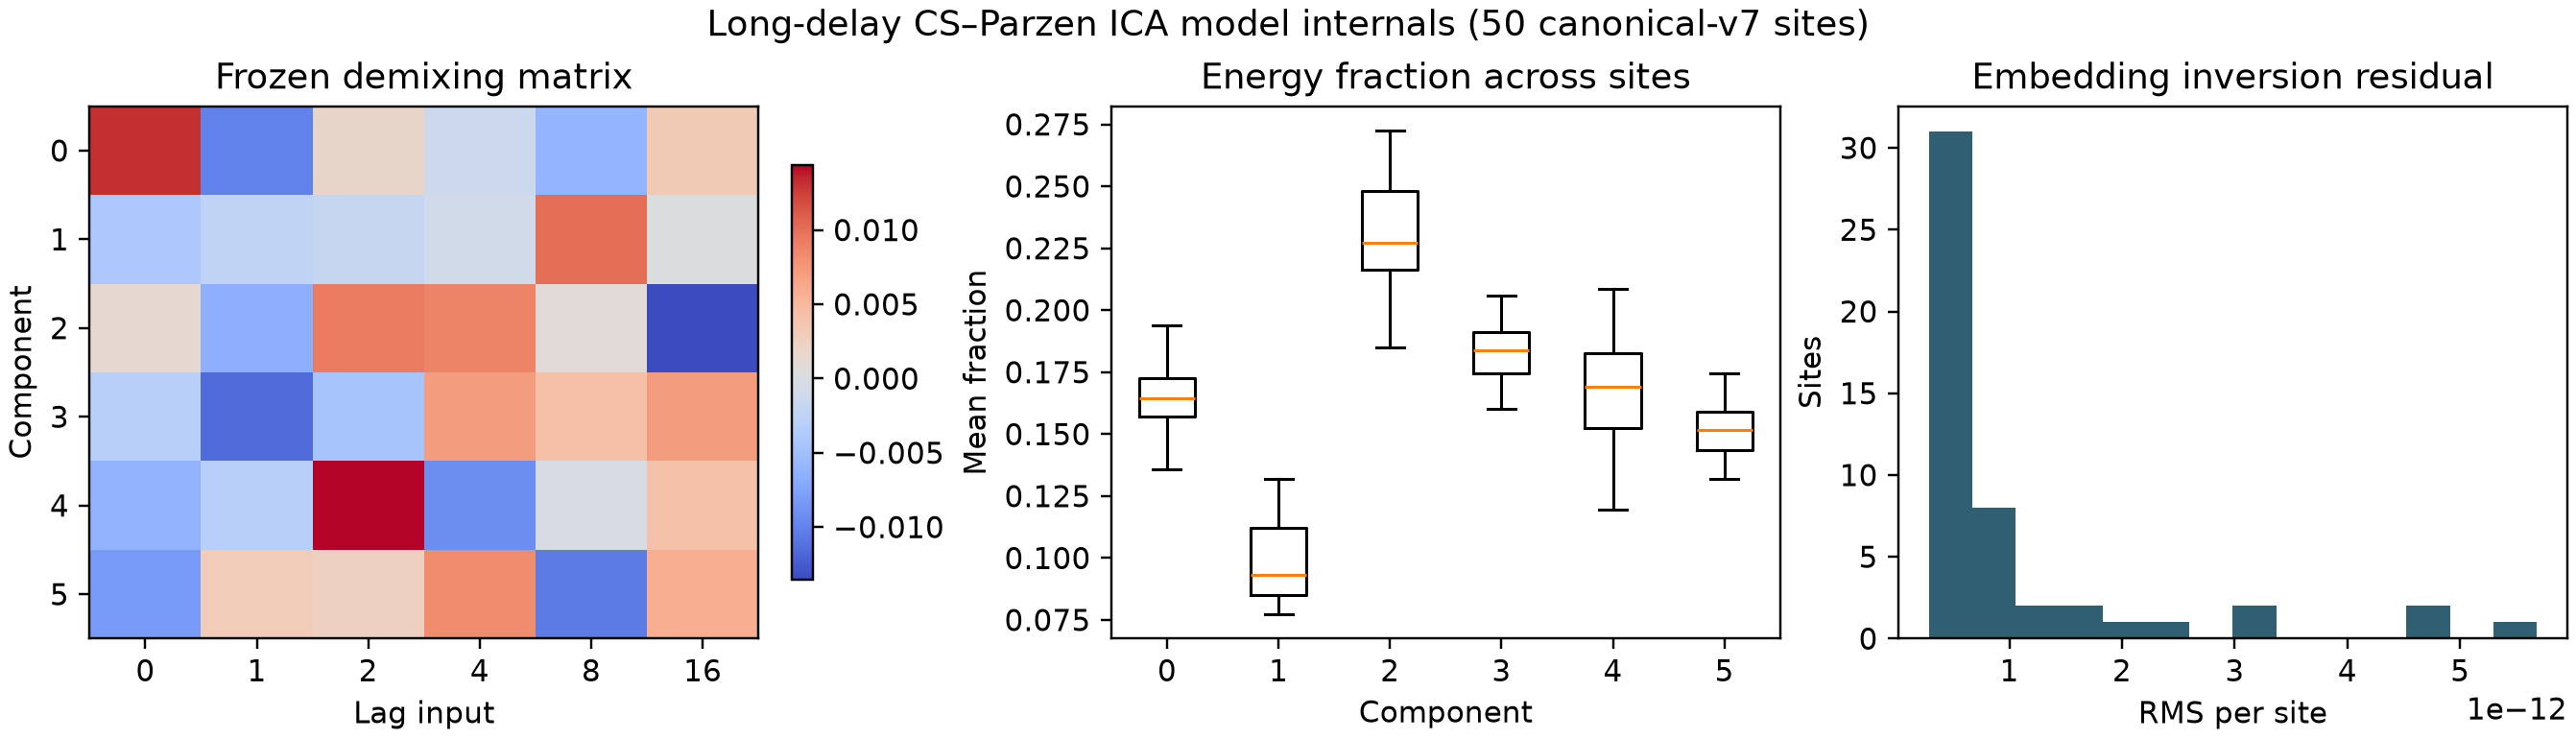
\includegraphics[width=0.98\linewidth]{figures/final/fig06_ica_model_internals.png}
  \caption{Frozen temporal-ICA internals. Component energy is distributed
  across the six outputs, and numerical inversion is accurate to floating-point
  precision.}
  \label{fig:overview-ica}
\end{figure}

The exact local-standardization denominator was reproduced using the frozen
fit, the original 31-frame causal pre-roll, the union of each site's 15-by-15
support, and the saved global scale floor (\Cref{fig:overview-denominator}). The
reproduced center outputs agree with the saved CUDA movie with RMS error
$6.96\times10^{-7}$. The floor is 0.371705, the median audited denominator is
0.7648, and the floor is inactive at every audited center. This makes the
interpretation more concrete: local-standardization strength at these centers
tracks measured local variability rather than a fallback constant.

\begin{figure}[p]
  \centering
  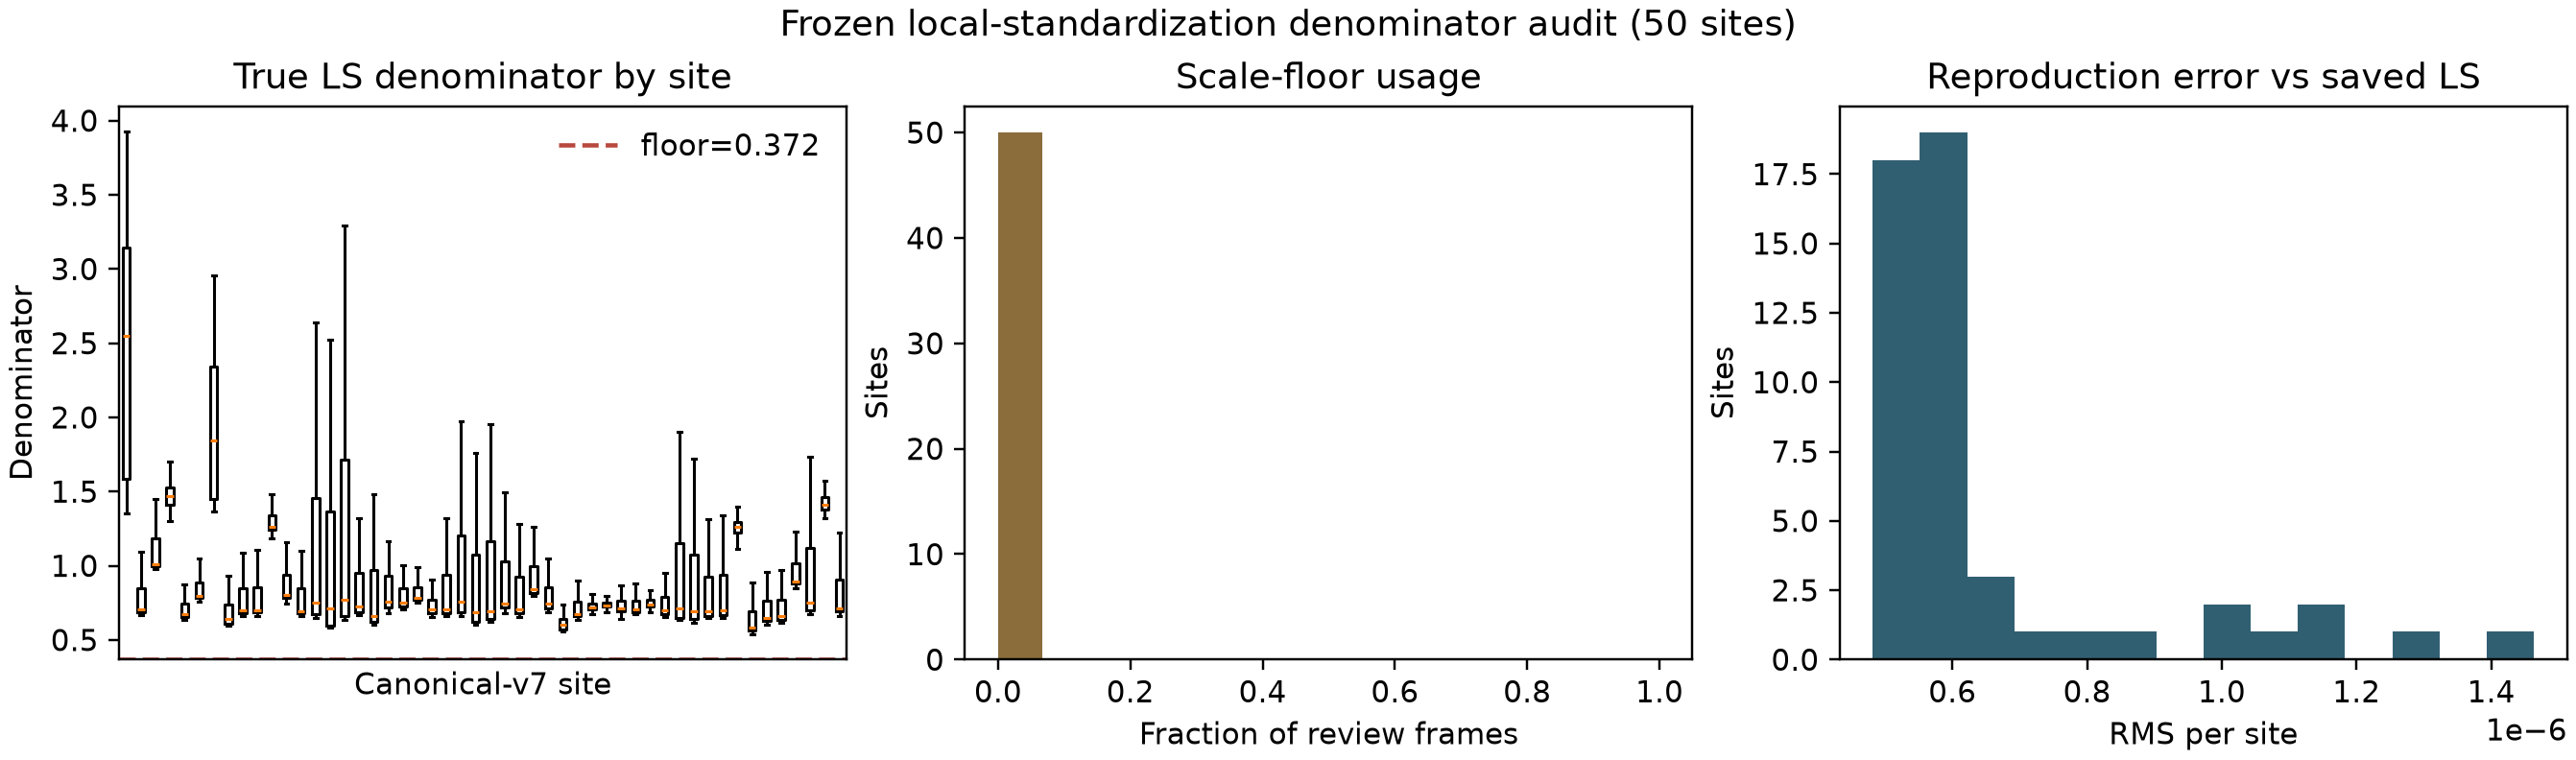
\includegraphics[width=0.98\linewidth]{figures/final/fig07_ls_denominator_diagnostics.png}
  \caption{True local-standardization denominator audit at 50 sites. Floor
  inactivity is established at the audited centers only, not across every pixel
  in the field.}
  \label{fig:overview-denominator}
\end{figure}

\section{How to interpret the research}

The most defensible interpretation is that this pipeline is sophisticated and
auditable feature engineering. Raw fluorescence preserves information but mixes
shared and local effects. Temporal ICA reorganizes lagged dynamics into a
stable coordinate system. Local standardization then expresses those dynamics
relative to recent neighborhood variability. Together they can improve
visibility and candidate ranking without guaranteeing that an output is an
independent neuronal source.

The expanded automated program has now exhausted the highest-value
same-recording checks. The next phase should be organized around three major
changes in evidence rather than additional small feature variants:

\begin{enumerate}
  \item \textbf{Independent frozen transfer.} Acquire or identify a second
  recording and apply the complete frozen pipeline, feature definitions,
  abstention rule, anomaly score, and identity-aware audit without retuning.
  This is the decisive test of whether observability context and failure
  structure generalize beyond the current fish and acquisition.
  \item \textbf{Identity-complete bounded truth.} Exhaustively adjudicate one
  bounded field with explicit distinct, overlapping, duplicate, uncertain, and
  non-neuronal states. This enables precision, identity-aware NMS, calibrated
  abstention, and a valid distinction between new discoveries and false
  positives.
  \item \textbf{Realistic generative movie validation.} Build a simulator with
  anatomy, overlapping footprints, optical blur, motion, indicator kinetics,
  shared drive, and sensor noise. Exact source identity will permit causal
  stress tests of carrier/context features, source separation, proposal
  formation, and identity-aware candidate selection.
\end{enumerate}

\section{Bottom line}

The current work establishes a reproducible measurement story: shared burst
dynamics are strong, local context matters, two recurring trace phenotypes are
visible, the frozen temporal transform is inspectable and numerically
invertible, and local standardization is governed by observed neighborhood
variability at the confirmed centers. Complete-trace analysis further shows
that amplitude nearly saturates known-center event localization, whereas
coherence is most useful upstream for candidate ranking. Automated challenge
tests confirm event alignment and localized measurement structure, but do not
confirm incremental recovery-model utility. It does not yet establish biological
source identity, independent-recording generalization, motion-free signal, or
full-field precision. Those are now sharply defined validation targets rather
than hidden assumptions.

\section*{Declaration of competing interests}
\AuthorDecision{Confirm that the authors have no competing financial or personal interests, or provide the required disclosure.}

\section*{Ethics statement}
\AuthorDecision{Insert the animal-use protocol, approving institution, protocol number, and confirmation that procedures followed applicable guidelines. Do not infer these details from the repository.}

\section*{Funding}
\AuthorDecision{List funding sources, grant numbers, and the role of each funder.}

\section*{CRediT authorship contribution statement}
\AuthorDecision{Complete CRediT roles for every author. Suggested roles to review include Conceptualization, Methodology, Software, Validation, Formal analysis, Investigation, Data curation, Visualization, Writing--original draft, Writing--review \& editing, Supervision, Project administration, and Funding acquisition.}

\section*{Data availability}
The release manuscript will cite a versioned data and annotation package or state the access restrictions and their justification. At minimum, the package will include immutable observation identifiers, site geometry, canonical-identity decisions, burst intervals, annotation provenance, configuration files, source hashes, generated result macros, and a figure/table source map. \AuthorDecision{Select public repository/accession, controlled-access process, or justified non-release statement.}

\section*{Code availability}
The analysis code will be released from a versioned NeuRev Workbench revision together with an executable environment specification and the protected-run configuration. \AuthorDecision{Insert repository URL, release tag, and archival DOI when available.}

\section*{Acknowledgements}
\AuthorDecision{Acknowledge data collectors, annotators, imaging collaborators, laboratory support, and computing resources.}

\section*{Declaration of generative AI and AI-assisted technologies in the writing process}
During manuscript preparation, the authors used OpenAI language-model tools to help organize the analysis plan and draft a manuscript skeleton. The authors are responsible for verifying all text, code, citations, numerical results, and interpretations and will review and edit the final submission. \AuthorDecision{Revise this disclosure to match the journal's submission form and the tools actually used in the final manuscript.}


\end{document}
